\documentclass{article}
\usepackage[margin=1.75in]{geometry}
\usepackage[utf8]{inputenc}
\usepackage{url}
\usepackage{hyperref}
\usepackage[backend=biber]{biblatex}
\usepackage{graphicx}
\usepackage{titlesec}
\usepackage{amsfonts}
\usepackage{amsmath}
\usepackage[table,xcdraw]{xcolor}
\usepackage{float}
\restylefloat{table}

\definecolor{tblgrey}{gray}{0.95}

\setcounter{secnumdepth}{4}

\titleformat{\paragraph}
{\normalfont\normalsize\bfseries}{\theparagraph}{1em}{}
\titlespacing*{\paragraph}
{0pt}{3.25ex plus 1ex minus .2ex}{1.5ex plus .2ex}

\addbibresource{Research.bib}

\title{Instant Messaging in the Blockchain}
\author{Jasper Parish}
\date{3\textsuperscript{rd} December 2019}

\begin{document}

\maketitle
\begin{abstract}
    An entirely decentralised, blockchain-based messaging service would allow for private and secure messaging whilst avoiding the hoarding of users' personal information by large companies. If the feature-set of a typical non-secure messaging app could be implemented into this decentralised system, then a competitive messaging service could be created that avoids nearly all the pitfalls of traditional messaging applications. This project describes, in great detail, the planning, research and design of a specification for the structure of the proposed blockchain; and the proposed network protocol.
\end{abstract}

\newpage
\tableofcontents
\newpage

\section{Research}
\subsection{The Problem}
The collection of user-data through various social-media, messaging and advertisement platforms has become the norm for many large companies. Many of these companies will hoard our data in their servers, possibly even selling it off to other businesses for profit. Privacy is a massive issue in the ethics of the tech community and I take the stance that we should protect our privacy at any cost. The revelations of the global population after Edward Snowden's leaks only make this issue more important. I do not believe that people should be tracked in a complete surveillance state, where the authorities can know your every move and everything you say or do is being watched. Messaging is a particularly important part of online social connections that I believe we should strive to keep secure.

\subsubsection{Proposed Solution}
Instead of giving power to major companies, I propose that we instead design a decentralised messaging platform that utilises blockchain technology to bring the features of all major instant-messaging apps to a decentralised world.

My proposal will allow people, who wish to, to take back ownership of their data. It will allow users to send anonymous messages to each other with the certainty\footnote{There is always some uncertainty, however, due to the state of cryptography and the nature of encryption.} that no one is able to intercept and read them.

This would also allow those who are locked in oppressive regimes or societies (that monitor/censor communication) such as that of North Korea to be able to communicate with external aid.

\newpage
\subsection{Planning}
Since this is quite a complex, large project, it will be important to carefully organise and manage my time and workload so as not to exceed deadlines.

\subsubsection{Project Breakdown}
The following is a breakdown of the project which I have planned to undertake. Though the final project will most probably deviate slightly due to unforeseen discoveries etc.

\begin{enumerate}
    \item Planning
    \begin{enumerate}
        \item Complete PPF
        \item Decide on exact sections of project
        \item Create Gantt chart for timings of each section and subsection
    \end{enumerate}
    \item Research
    \begin{enumerate}
        \item Complete research and notes on the following topics:
        \begin{enumerate}
            \item What is Bitcoin and how does it work?
            \item What is Bitcoin's implementation of blockchain?
            \item What is Bitcoin's implementation of a peer-to-peer network
            \item What are the simple cryptographic algorithms used in blockchains and how do they work? (Hash functions etc.)
            \item What are the more advanced cryptographic algorithms and how do they work? (signatures etc.)
            \item What is elliptic curve cryptography and how does it work?
            \item What are the advantages and disadvantages of the Bitmessage platform?
            \item How can you minimise block-times and how far can you go?
            \item What is proof-of-stake and is it useful to this project?
            \item How can addresses be made that are easy to work with?
            \item How could you transition the blockchain from being designed for currency to being designed to carry messages?
            \item What are the ethics of the proposed platform?
            \item How do privacy coins differ from Bitcoin.
            \item How can the client maintain low resource intensity when interacting with the blockchain.
        \end{enumerate}
        \item Compile into research report write-up.
    \end{enumerate}
    \item Design and Development
    \begin{enumerate}
        \item Blockchain architecture design
        \item P2P network protocol design
        \item Code proof-of-concept application
    \end{enumerate}
    \item Evaluation - TBC
\end{enumerate}


\subsubsection{Time management}
To manage my time over the weeks of research, I have created a Gantt chart. This got modified throughout my research as I found that some topics required more or less time than previously expected.
\begin{figure}[h]
    \centering
    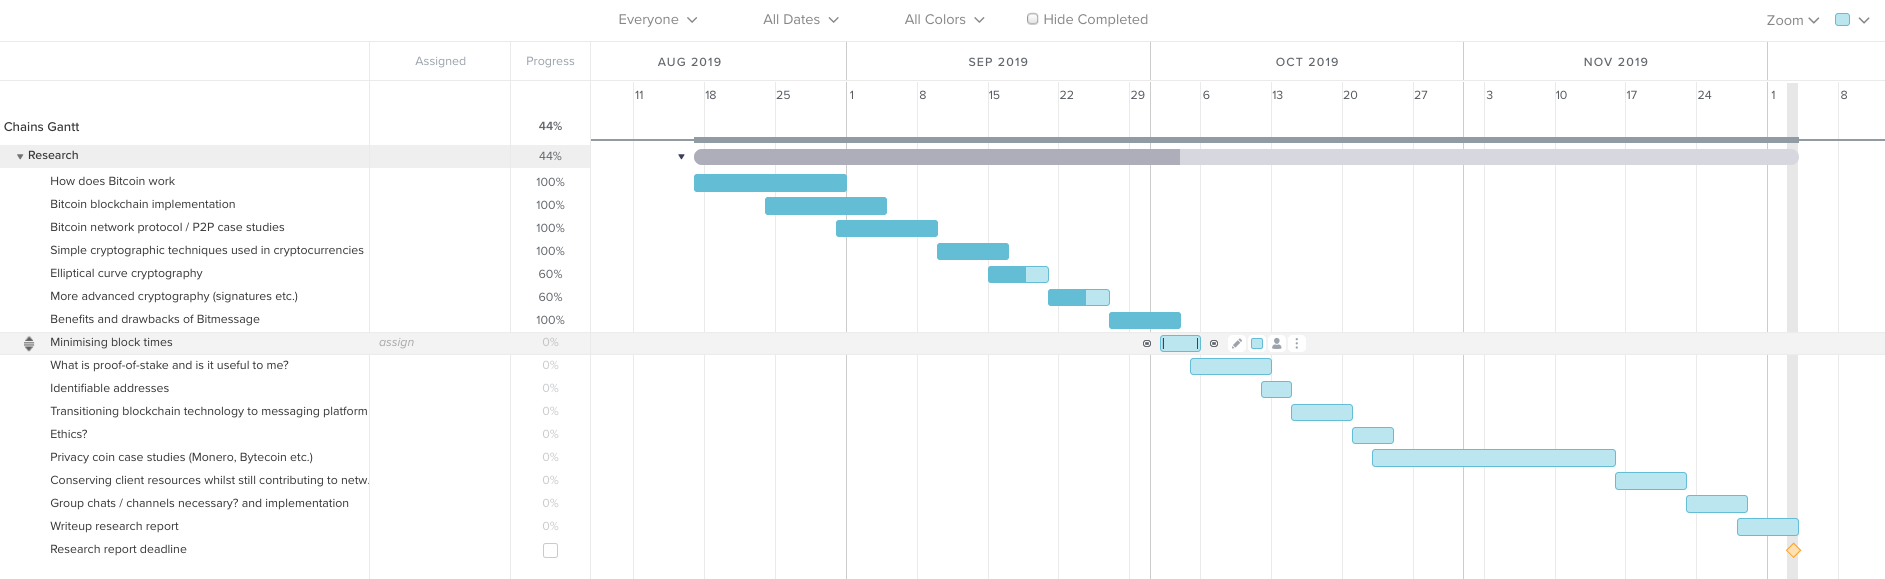
\includegraphics[width=0.9\linewidth]{Images/Gantt_before_ec.png}
    \caption{My original research Gantt chart that I made at the start of the project.}
    \label{fig:ganttbefore}
\end{figure}
\begin{figure}[h]
    \centering
    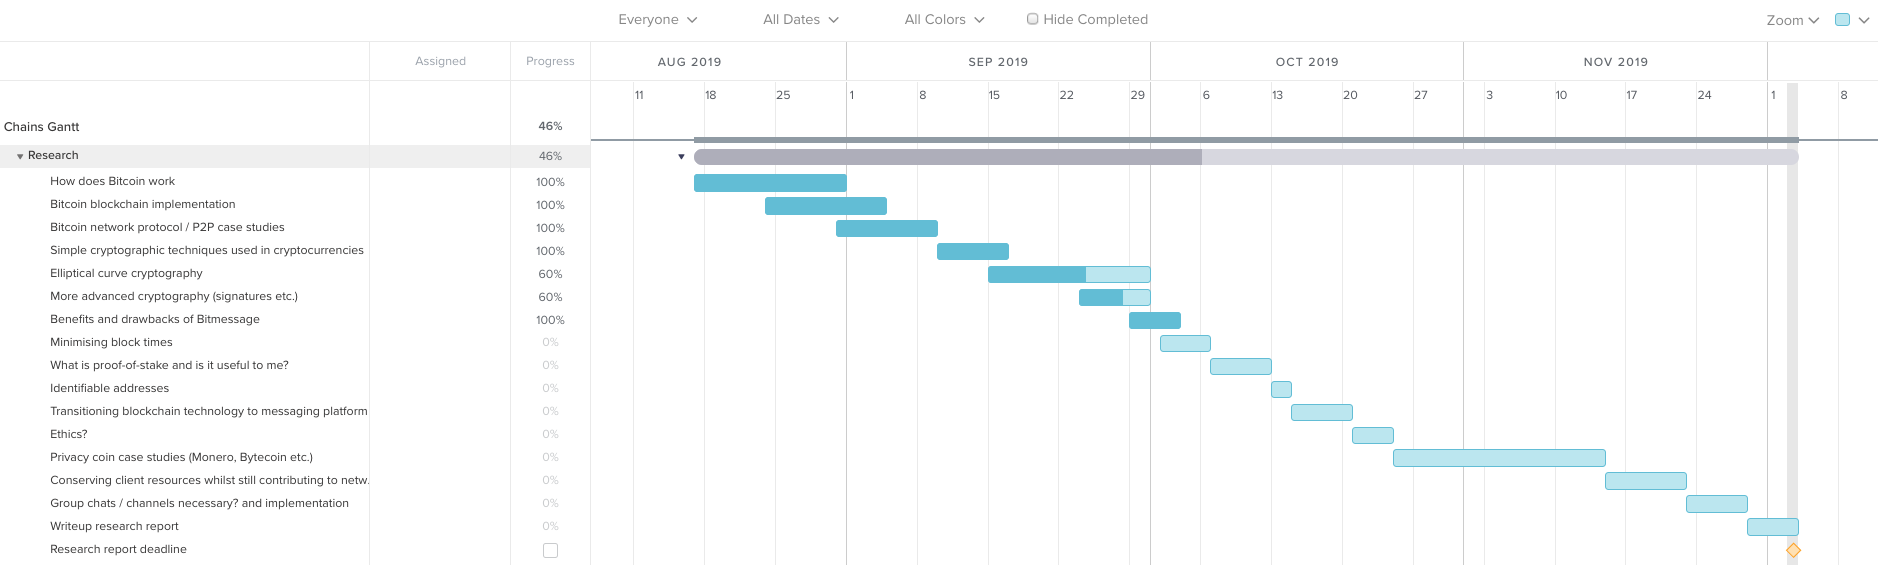
\includegraphics[width=0.9\linewidth]{Images/Gantt_after_ec.png}
    \caption{My research Gantt chart, modified after having realised that Elliptic curve cryptography is a much more complex topic than I previously thought.}
    \label{fig:terec}
\end{figure}

The day after the deadline, I realised that I had neglected to properly discuss ``Minimising Block Times'' which is an important but small part of the project.
\begin{figure}[h]
    \centering
    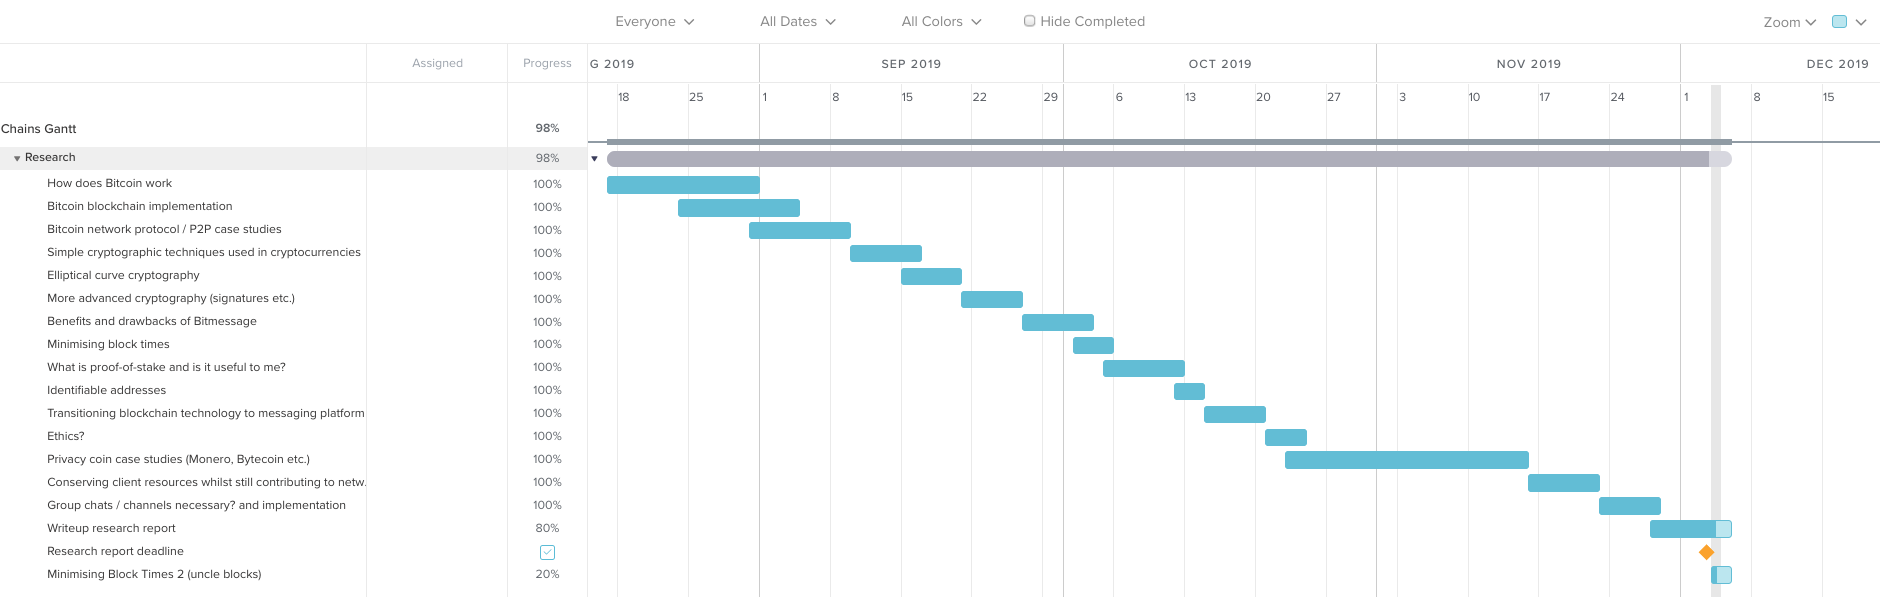
\includegraphics[width=0.9\linewidth]{Images/Gantt_after_uncle.png}
    \caption{My research Gantt chart, modified after having realised that I had not properly discussed ``Minimising Block Times'' in my write-up.}
    \label{fig:teruncle}
\end{figure}
\newpage


\subsection{Why Blockchain?}
The vast majority of messaging platforms at the moment utilise a simple client-server model to allow communication between users. Although this works well for a messaging system, it has several arguably major drawbacks which will be discussed in the next few pages.

\subsubsection{Messaging Case Study - Facebook Messenger / Whatsapp}
Both Facebook Messenger and Whatsapp are feature-packed messaging apps that provide the user with an excellent messaging platform allowing users to quickly and reliably communicate. Globally, over 3bn people use Whatsapp or Facebook Messenger every month, making these 2 platforms the most popular of any in the world.
\begin{figure}[h]
    \centering
    
\includegraphics[width=0.4\linewidth]{Images/fbmsgwhtspp.jpeg}
    \caption{Facebook messenger (left) and Whatsapp (right) are the two leading messaging platforms globally.}
    \label{fig:fbmsgwhtspp}
\end{figure}
However, they rely on the client-server model. This means that all messages are stored on servers in a data-centre. Even though these companies say that all messages are encrypted, it is not guaranteed that they are. In fact, many people believe that the USA's National Security Agency (and other nations' governments) has been granted 'back doors' into the platforms. This would potentially allow authorities to spy on the general population and results in the loss of privacy for billions of people. I strongly disagree with even the possibility of this being the case as I value my privacy greatly. I believe that everyone should have access to free-speech and privacy.
Also, storing users' data on servers poses a security risk since most of these platforms are completely proprietary and not open source. Servers could potentially be hacked leading to the distribution of user data across illegal forums and marketplaces. This could happen without even the companies' knowledge and bypasses any GDPR data regulations. This shows that these platforms, whilst feature-packed and easy-to-use, are not necessarily trustworthy in the current age of privacy and data-protection.

\subsubsection{Messaging Case Study - Bitmessage}
Bitmessage\cite{bitmessage_paper} is a decentralised messaging platform that runs on a global peer-to-peer network. Messages are each individually encrypted and distributed across the network. Each machine (completely voluntarily) supports the network by echoing new messages to all its known neighbours.
\begin{figure}[h]
    \centering
    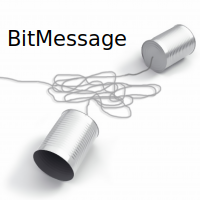
\includegraphics[width=0.4\linewidth]{Images/bitmessagelogo}
    \caption{The Bitmessage logo}
    \label{fig:bitmessagelogo}
\end{figure}
The idea of Bitmessage is very strong and manages to achieve pseudonymity whilst also being decentralised. This means that, similar to Bitcoin, all addresses for users of the network are not linked to real people. However, unlike Bitcoin, there is no single source of truth. This means that when a user wants to check if they have received any messages, they download a message-pool (a large-group of cached messages) from some of their peers on the network and check for any which were created using their public key. This means that the sender cannot confirm for certain that the recipient will have access to the sent message and can only hope that that the message makes its way across the network. Although this is not a platform-breaking issue, it could be very significant in situations that rely on reliable, consistent messaging.
One of the great inventions of the Bitmessage platform is the idea of proof-of-work for individual messages. This effectively eliminates spam on the network by making every message require the sender to give up computational resources (users who try to overload the network with messages will have to dedicate unreasonable amounts of computational power to the creation of large quantities of messages).
However, another downside of Bitmessage is the slow propagation delay. Bitmessage is often likened to email due to the way it has been implemented. Messages are treated like emails rather than a persistent instant chat. This means that correspondence with recipients could be slow and disjointed.

\subsubsection{Blockchain Case Study - Bitcoin}
Bitcoin\cite{bitcoin_paper} is the first notable implementation of blockchain technology and was the first blockchain-based cryptocurrency ever. It is useful to examine Bitcoin as one can see the design decisions behind the architecture of a cryptocurrency. Since nearly all other cryptocurrencies adapt their system from Bitcoin in some way, this gives a good view of the basis for a cryptocurrency and how a blockchain should work. It is also simpler than many other cryptocurrencies making it easier to investigate and understand. Bitcoin has become so popular that many shops around the world now accept the currency in shops IRL (see \autoref{fig:bitcoinacceptedhere}) and not just on the internet.
\begin{figure}[h]
    \centering
    
\includegraphics[width=0.5\linewidth]{Images/bitcoin_accepted_here.png}
    \caption{A sign created for sellers to show acceptance of bitcoin as payment method}
    \label{fig:bitcoinacceptedhere}
\end{figure}
For its time, bitcoin was innovative in its privacy for users. It circumvented the need for accounts like PayPal and Stripe do today. It did this using some clever cryptography that allowed for trustless interaction. However, the Bitcoin blockchain is vulnerable to so-called ``blockchain-analysis''. This entails some users tracing and cross-referencing transactions and addresses over a long period, eventually resulting in compromised user identities. This practice could be carried out by governments or private agencies to bypass the layer of anonymity that stands in-between user's and their wallet addresses. This layer of psuedo-anonymity is known as pseudonymity and has since been deemed less-than-private by the cryptocurrency community.

\subsubsection{Blockchain Case Study - Monero}
Monero (built on Cryptonote\cite{cryptonote_paper}) is currently (as of Nov. 2019) the most popular of all the so-called ``privacy coins''. Cryptonote and consequently Monero are built with the premise of true-anonymity in mind. They utilise some more complex cryptography in order to hide the addresses of senders and recipients. This involves ``stealth-addresses'', which are alias addresses used by the recipient of a payment, and ring signatures which preserve the identity of the message sender whilst simultaneously hiding the quantity of currency in each transaction (Ring CTs).
\begin{figure}[h]
    \centering
    
\includegraphics[width=0.4\linewidth]{Images/monerologo.png}
    \caption{The Monero logo}
    \label{fig:monerologo}
\end{figure}
In terms of using the payment framework itself, the currency is just as easy for users to use as Bitcoin. Monero is probably the most well-backed privacy coin with the best documentation. \url{GetMonero.org} (the official Monero website) has many videos and blog posts explaining all the aspects of the currency. 

The Monero Project has also kick-started The Kovri Project\cite{kovri_repo}. This is a new system for routing and encrypting network traffic in peer-to-peer networks such as Monero's. This could be useful to my project as the security of the network is theoretically just as important as the security of the blockchain/ledger itself.


\subsubsection{Blockchain as a Solution}
A blockchain would provide a single source of truth for all messages on the network meaning that, for the most part, all machines on the network will be in agreement over all messages. This means that there should never be a situation where a message is lost before it is accessible to the recipient. Blockchains are effective for this solution because they group together message 'transactions' making a shared database that anyone can access and anyone can store for as long as they wish. Blockchain does have some downsides however. For example, they are not really designed to work at high block frequency (more blocks found per minute) and will become inherently less secure when at the higher speeds required for an instant messaging service. This will need to be addressed clearly later on if this service is to be considered remotely secure.

This system means that individual mobile devices can store the blockchain on their hard drives and be sure of its authenticity to a great deal of certainty. This does, however, introduce the problem of scalability as storing a ledger of all messages ever sent on the network will quickly become impractical.

\subsection{What is (a) Blockchain?}\label{subsubsec:whatisablockchain}
A blockchain is essentially a database that stores a set of grouped records (rows in a data set). These groups of records are known as blocks and each record is typically some form of transaction (in the case of cryptocurrencies, these are monetary transactions). However, it should be noted that these records could be used for a multitude of different uses including digital electoral votes; gambling bets; and medical records. Each block of records contains a reference to the previous block, creating a chain.

Blockchains are most useful when distributed between many computers on a network. This is because they can be combined with some cryptography to allow for trustless interaction between users of the blockchain. The concept of trustless interaction with blockchains is explained well in a blog-post from 2018\cite{medium_trustless_blockchain}. The classic example for this is the transfer of money between two parties. 
\begin{figure}[h]
    \centering
    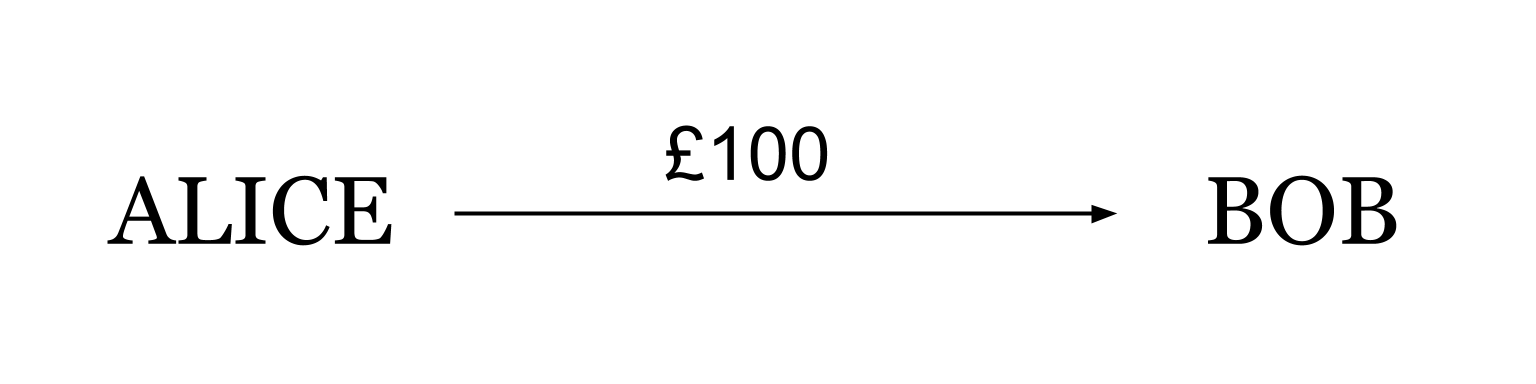
\includegraphics[width=0.65\linewidth]{Images/Diagrams/transaction_in_person.png}
    \caption{Alice gives £100 to Bob in person}
    \label{fig:transactionwoip}
\end{figure}
As explained in the blog-post, the easiest and simplest way to transfer money would be for the two parties to meet in person and trade physical money (see \autoref{fig:transactionwoip}). However, this is not always possible for people who are in either remote location or for those who don't trust their opposite party. One solution to this is to have a trusted intermediary party (usually a bank) who could facilitate the transaction (see \autoref{fig:transactionwip}). 
\begin{figure}[h]
    \centering
    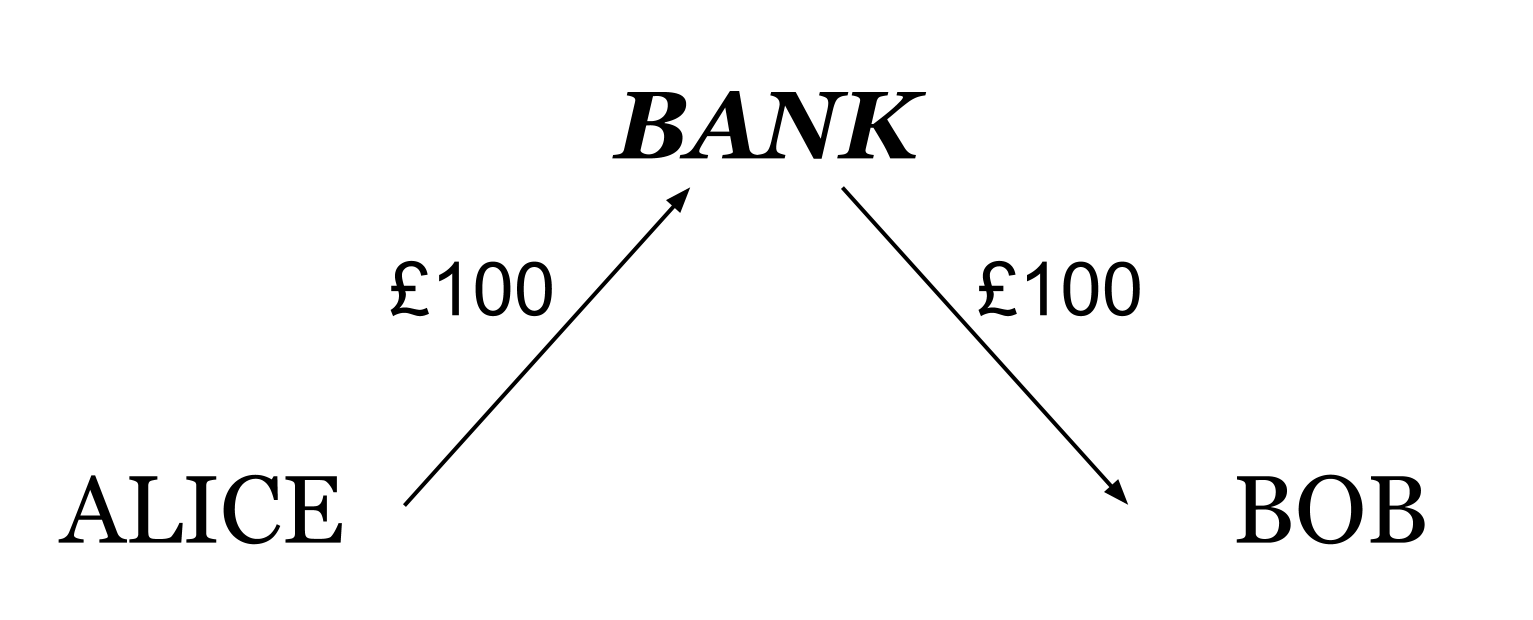
\includegraphics[width=0.65\linewidth]{Images/Diagrams/transaction_with_intermediary.png}
    \caption{Alice sends £100 to Bob through an intermediary party}
    \label{fig:transactionwip}
\end{figure}
This is ideal in the sense that both parties can safely partake in transactions without the drawbacks of meeting up in person. This solution is the most popular of all and is well-established in the global economy. However, once again, there are several drawbacks associated with this form of transaction. Firstly, how can a party be absolutely sure that their intermediary party is in fact trustworthy. This can become quite problematic when large sums of money are being transacted. Also most intermediary parties (banks) are obligated to decline the facilitation of transactions that are believed to be illegally premised or against their wishes. Moreover, if a bank logs all of its transactions, then the private data of the user can be hoarded and sold on for the intermediary's profit. As well as this, if the intermediary party were to shutdown or go bankrupt, then the user's money could be lost altogether and the transaction would fail. Cryptocurrencies solve this problem by replacing the intermediary party with a blockchain.
\begin{figure}[h]
    \centering
    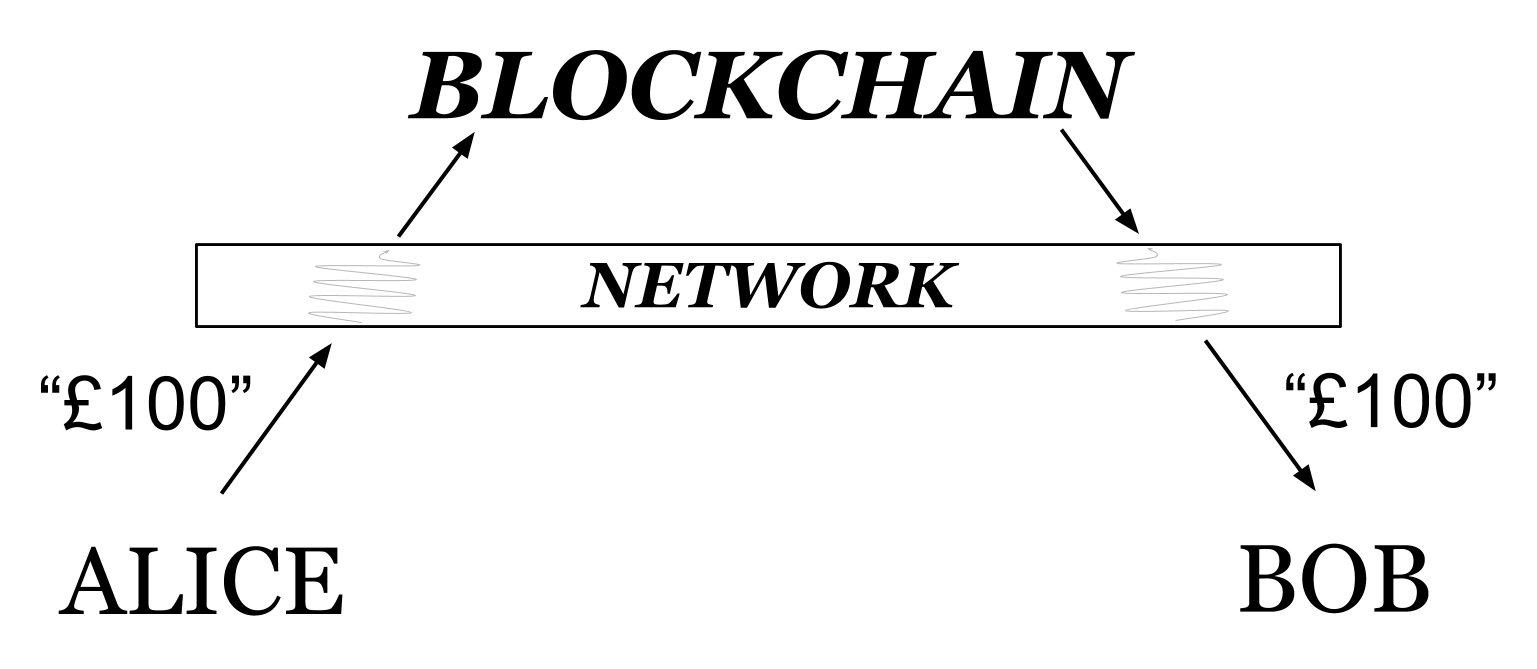
\includegraphics[width=0.65\linewidth]{Images/Diagrams/transaction_with_blockchain.png}
    \caption{Alice sends £100 by means of a blockchain}
    \label{fig:transactionwbc}
\end{figure}
Instead of sending payments to a bank (or other intermediary), a user would declare to a network of listening computers that they wish to make a payment and these computers would record it in the blockchain (see \autoref{fig:transactionwbc}).
These nodes (computers) on the network would always validate a transaction before allowing it to become part of the blockchain. This way, no one is able spend money that they do not have. The network of computers is always running and all connections are direct internet connections between IP addresses. 
Communication is between peers rather than between client devices and centralised servers and is the reason that the network is known as peer-to-peer (rather than client-server as in most contemporary internet communication, see \autoref{fig:p2pnetwork}). New peers are welcomed to the network at any time and likewise anyone can leave. It should be noted, however, that when only a few peers are online in the network, the network will seem to be slow as many connections are being routed through only a few nodes.
\begin{figure}
    \centering
    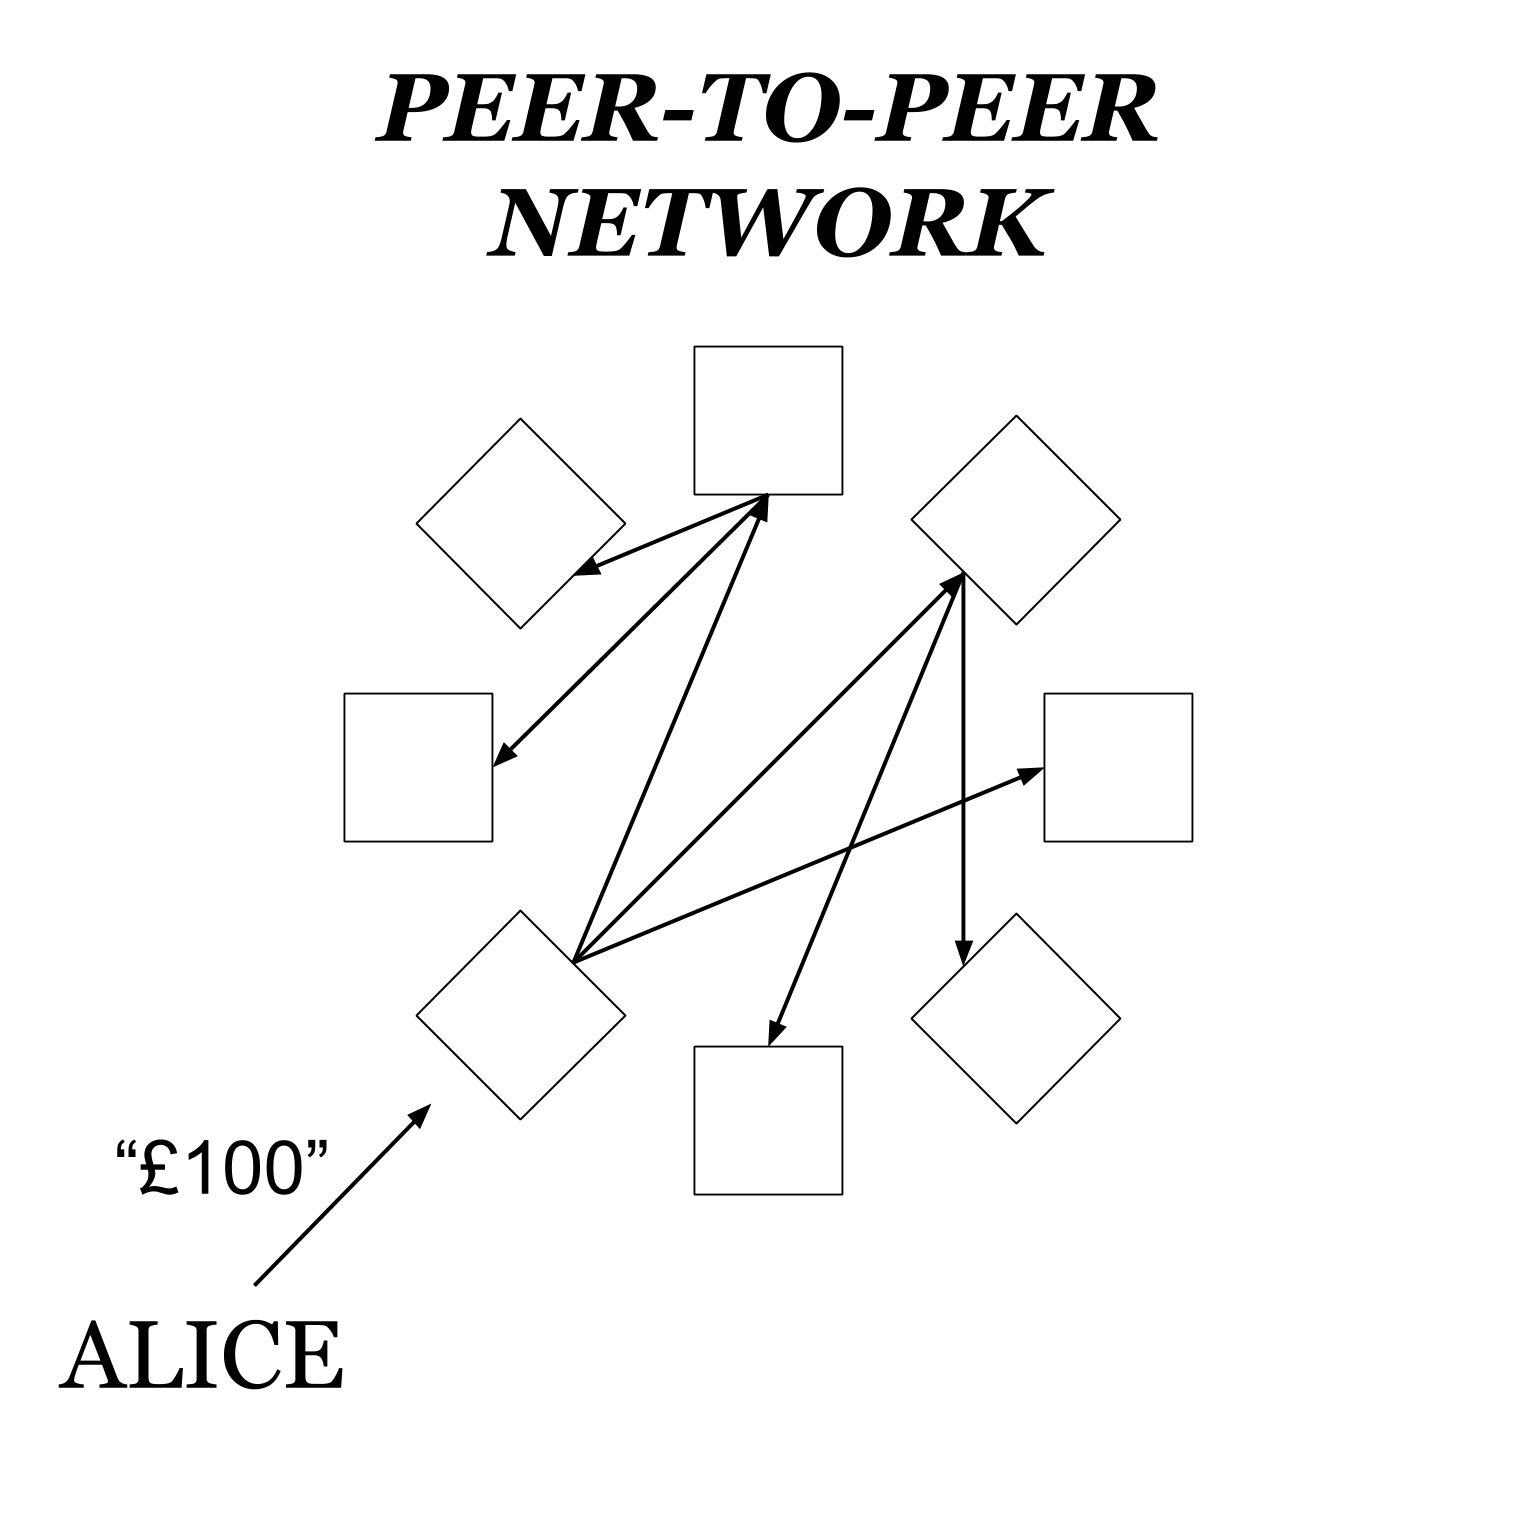
\includegraphics[width=0.5\linewidth]{Images/Diagrams/p2p_network.png}
    \caption{Alice sends the details of her transaction into the peer-to-peer network}
    \label{fig:p2pnetwork}
\end{figure}

When computers on the network receive a transaction, they first confirm the validity of the transaction against the user's previous outputs (received payments, this is a way of checking wallet balance). They then group this with a large number of other recently received transactions between other parties. They then attempt to solve a mathematical puzzle known as a proof-of-work (first proposed for the blockchain in the Bitcoin white paper\cite{bitcoin_paper}). All the nodes on the network will use their computational power to try to break the puzzle and the first one to do so will broadcast their found block to the network. This newly created block contains all the transactions that the solver grouped in the previous step and also the solution to the puzzle. This allows anyone on the network to validate the block by quickly checking if the solution is correct. If a node validates the block, it will add it to its copy of the blockchain. If not, then the node will reject it. The difficulty of the puzzle is adjusted every so often to make sure that the time between blocks being 'found' (the moment when a solution is found to a puzzle and the block is posted) is fairly constant (in Bitcoin and Monero's case, the block-times are around 10 minutes and 10-20 seconds respectively). Nodes on the network follow strict communication rules known as the network protocol (Bitcoin\cite{bitcoin_docs} and Bitmessage\cite{bitmessage_docs}).

Since every block on the blockchain points to the block that came before it, the longest chain of blocks is assumed to be truth. This chain has had the most computational work put into it, since the most puzzles have been solved and thus is most likely to be truth. The longer the chain, the more secure users can be in the knowledge that their transactions are safe. Traditionally (in Bitcoin, Monero and other cryptocurrencies), these nodes are rewarded for dedicating their computing power towards supporting the network. This reward consists of a new piece of currency and is how new ``coins'' are introduced into the system.

\subsubsection{Scalability}
One of the greatest benefits of a peer-to-peer network is that it should become faster to use as more nodes join the network. This is very different to the client-server paradigm where companies are forced to spend more and more money on server infrastructure as network traffic increases.

However, pushing updates to servers is often a much easier task than persuading a global peer-to-peer network to do the same. This means that updates will often take longer (normally over a period of months, for example Bitmessage took over a month to upgrade its network to ``protocol v3''\cite{bitmessage_protocol_v3}). This could be a security issue if an exploit is found in the given protocol specification for a network. This means that great care must be taken when devising a network protocol.

Scalability was also a problem in the case of Bitmessage because of the way in which a user finds messages addressed to him; Bitmessage, requires every user to scan through all messages on the network attempting to decrypt every one until one is successfully decrypted. This could slow down message receipt as more messages enter the network and Bitmessage becomes more popular. However, it would compromise much of the network's anonymity to omit this and this may have to become part of the proposed instant messaging platform.

\subsubsection{Minimising Block Times}
Block times are the mean period of time between two adjacent blocks being discovered. In Bitcoin, the block times were set to be around ten minutes. This means that the difficulty of the mathematical puzzle is dynamically changed to keep the time between blocks fairly constant. The more nodes ``mining'' on the network, the more consistent and stable the block times should be since the difficulty will be higher and the probability of finding a block will be lower and spread out over many ``miners''.

Ethereum\cite{ethereum_intro_paper}, a more modern cryptocurrency than Bitcoin, uses block times of 10-20 seconds which means that the rate of finding blocks is significantly higher. This means that the time it will take for a transaction to enter the blockchain will be significantly lower than that of Bitcoin's. Since instant messaging requires fast communication, the proposed platform will require block times on the order of 10-20 seconds like Ethereum's.

''Difficulty'' in Bitcoin is recalculated every 2016 blocks (see \autoref{fig:bc_diff_eq}).
\begin{figure}[h]
    \[\textrm{difficulty}_{\textrm{new}} = \frac{\textrm{difficulty}_{\textrm{old}} \times (2016\ \textrm{blocks} \times 10\ \textrm{minutes})}{\textrm{total time taken (mins) to mine last 2016 blocks}}\]
    \caption{Equation to calculate difficulty (as deviation from original (1.00)) for Bitcoin.\cite{medium_bt_mystery}}
    \label{fig:bc_diff_eq}
\end{figure}
%new_difficulty = old_difficulty X (2016 blocks X 10 minutes) / (the time took in minutes to mine the last 2016 blocks)

In Ethereum, difficulty is calculated ``on the fly''. This means that the difficulty is recalculated after every block and is constantly changing. This should be a more effective approach for the early stages of a blockchain since the fluctuations in total network hash rate from the norm are much more significant.

Difficulty in Ethereum is recalculated based on the most recent block time (see \autoref{fig:eth_diff_eq}).
\begin{figure}[h]
    \[\textrm{difficulty}_{\textrm{new}} = \textrm{difficulty}_{\textrm{old}}
    \ + \ \left\lfloor\dfrac{\textrm{difficulty}_{\textrm{old}}}{2048}\right\rfloor \times \max\left(1- \left\lfloor \frac{\textrm{block\_time}}{10} \right\rfloor,\ -99\right)\]
    \caption{Equation to calculate Ethereum's difficulty (Homestead release) ignoring the ``difficulty bomb''\cite{medium_bt_mystery}. ``block\_time'' is the difference in timestamps between the two most recently found blocks.}
    \label{fig:eth_diff_eq}
\end{figure}

As discussed at the start of \autoref{subsubsec:whatisablockchain}, nodes have to solve mathematical puzzles for the network to function. For Bitcoin and most other cryptocurrencies, the actual puzzle is defined as taking many hashes (see \autoref{subsubsec:hashfns}) of proposed blocks (each a set of transactions grouped by the node). Every block contains a ``nonce'' value. This is just an integer that is kept in the headers. This nonce is incremented after every hash calculation. If the hash of the block with the nonce was less than (or equal to) a specified target, then the block is valid and can be broadcast to the network. If it is greater than the specified target, then the nonce is incremented and the process repeated until either the target is met or a found block is received from the network. This process becomes very resource-intensive at high speeds so machines with a greater hash rate (processing speed) will be able to, on average, calculate more blocks over a period of time. This is known as ``mining'' and was first discussed (for blockchain) in Satoshi Nakamoto's Bitcoin proposal\cite{bitcoin_paper}. In Bitcoin, the network is so full of high hash-rate miners that it is no longer even remotely profitable to mine on a typical desktop machine. Other cryptocurrencies choose to implement hash functions that favour the processors available in more accessible machines (Monero uses the Cryptonight algorithm\cite{cryptonight_docs} which favours the CPU over high-power GPUs and so-called ASICS).

To calculate the target value, it is as simple as scaling the previous target according to the new difficulty (see \autoref{fig:target_eq}).
\begin{figure}[h]
    \[\textrm{target}_{\textrm{new}} = \frac{\textrm{target}_{\textrm{old}}} {\textrm{difficulty}_{\textrm{new}}}\]
    \caption{Equation to calculate target value from current and previous difficulties.}
    \label{fig:target_eq}
\end{figure}
This algorithm should theoretically not `care' about the initial target chosen so long as it is reasonably low difficulty (the system should self stabilise). 

%block_time=current_block_timestamp — parent_block_timestamp
%current_block_difficulty = parent_block_difficulty + (parent_block_difficulty // 2048) * max(1 — (block_time// 10), -99) + int(2**((current_block_number // 100000) — 2))


%new_target = old_target / new_difficulty


\paragraph{GHOST protocol}
Blockchains become inherently less secure when block times are low and this was the reason that Satoshi Nakamoto chose 10 minutes for Bitcoin rather than something much shorter. However, as previously mentioned, Ethereum's block times are significantly shorter (10-20 seconds). The topic of minimising block times is explained well by the creator of Ethereum, Vitalik Buterin, in a blog post\cite{toward_twelve_s_bt}. The reason that security that security suffers at low block times is due to the network propagation delay. Network propagation delay is the length of time between a found-block being broadcast and it being received by all\footnote{usually it is more useful to discuss 95\% of the network, rather than 100\% since the last 5\% are often \emph{very} slow.} of the network. As discussed in Bitcoin's proposal paper\cite{bitcoin_paper}, we can calculate the probability of an attacker having control of the network.

Take, for example, a blockchain on a network $N$ of the following properties:
\begin{align*}
    p &:= \textrm{probability an honest node finds the next block} \\
    q &:= \textrm{probability the attacker finds the next block} \\
    q_{z} &:= \textrm{probability the attacker will ever catch up from z blocks behind} \\
    D &:= \textrm{Network propagation delay} \\
    t_b &:= \textrm{Expected block time}
\end{align*}

If we consider the case where there is no propagation delay (ie. $D = 0$), then:
\[
q_z = 
\begin{cases}
    1                           &\textrm{if } p \leq q \\
    \left(\frac{q}{p}\right)^z  &\textrm{else}
\end{cases}
\]

As the attacker gets further behind on his parallel version of the blockchain, it becomes exponentially less likely for him to ever catch up. When not taking into account the propagation delay of the network, the blockchain can be modelled very simply. It is simply a series of successive blocks where each references the last (see \autoref{fig:blockchain_no_pdelay}).
\begin{figure}[h]
    \centering
    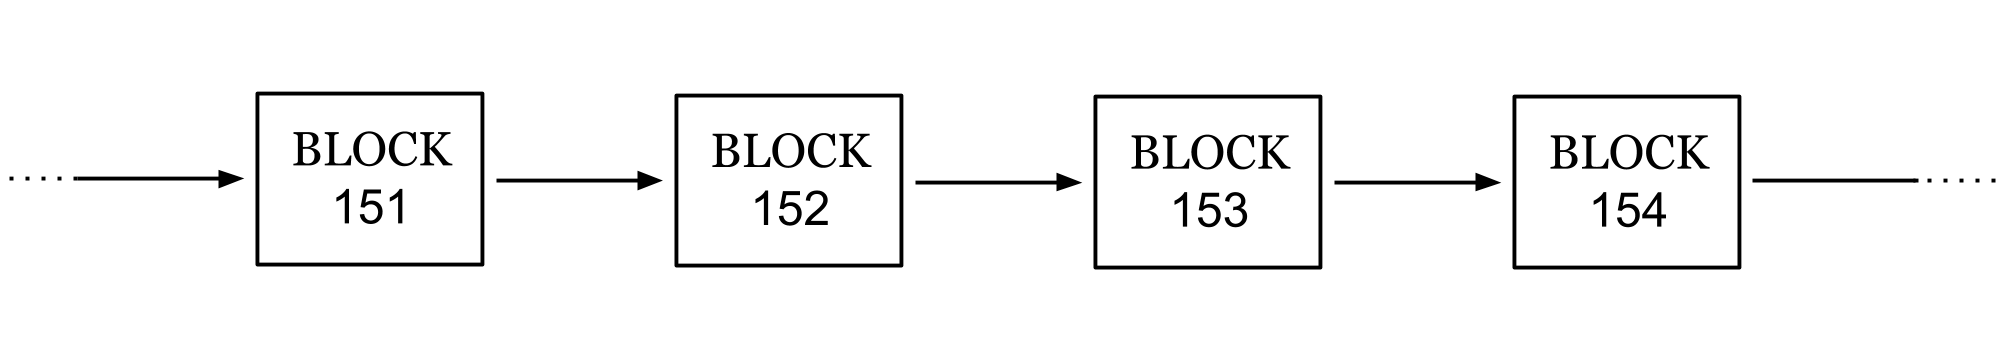
\includegraphics[width=0.9\linewidth]{Images/Diagrams/blockchain_no_pdelay.png}
    \caption{Simple model of a blockchain (not taking network propagation delay into account). Note that the arrows are reversed to show the child of a block rather than the referenced parent.}
    \label{fig:blockchain_no_pdelay}
\end{figure}

The issues of low block times arise when propagation delay \emph{is} taken into account. Now consider a network with a network propagation delay $D = 1$ minute and a expected block time $t_b = 10$ minutes. In such a network, every found block will take 1 minute to reach every node on the network. This means that another node, somewhere on the network, may continue mining for a minute longer than the first person to find the block. This also means that they may find a block before they receive knowledge of any other blocks (see \autoref{fig:blockchain_w_pdelay}). This block is known as a ``stale'' since some of the nodes on the network are aware of a block with an earlier timestamp. This introduces a weakness in the security of the blockchain as a whole because now an attacker is not required to have a majority in hash rate of the whole network.

\begin{figure}[h]
    \centering
    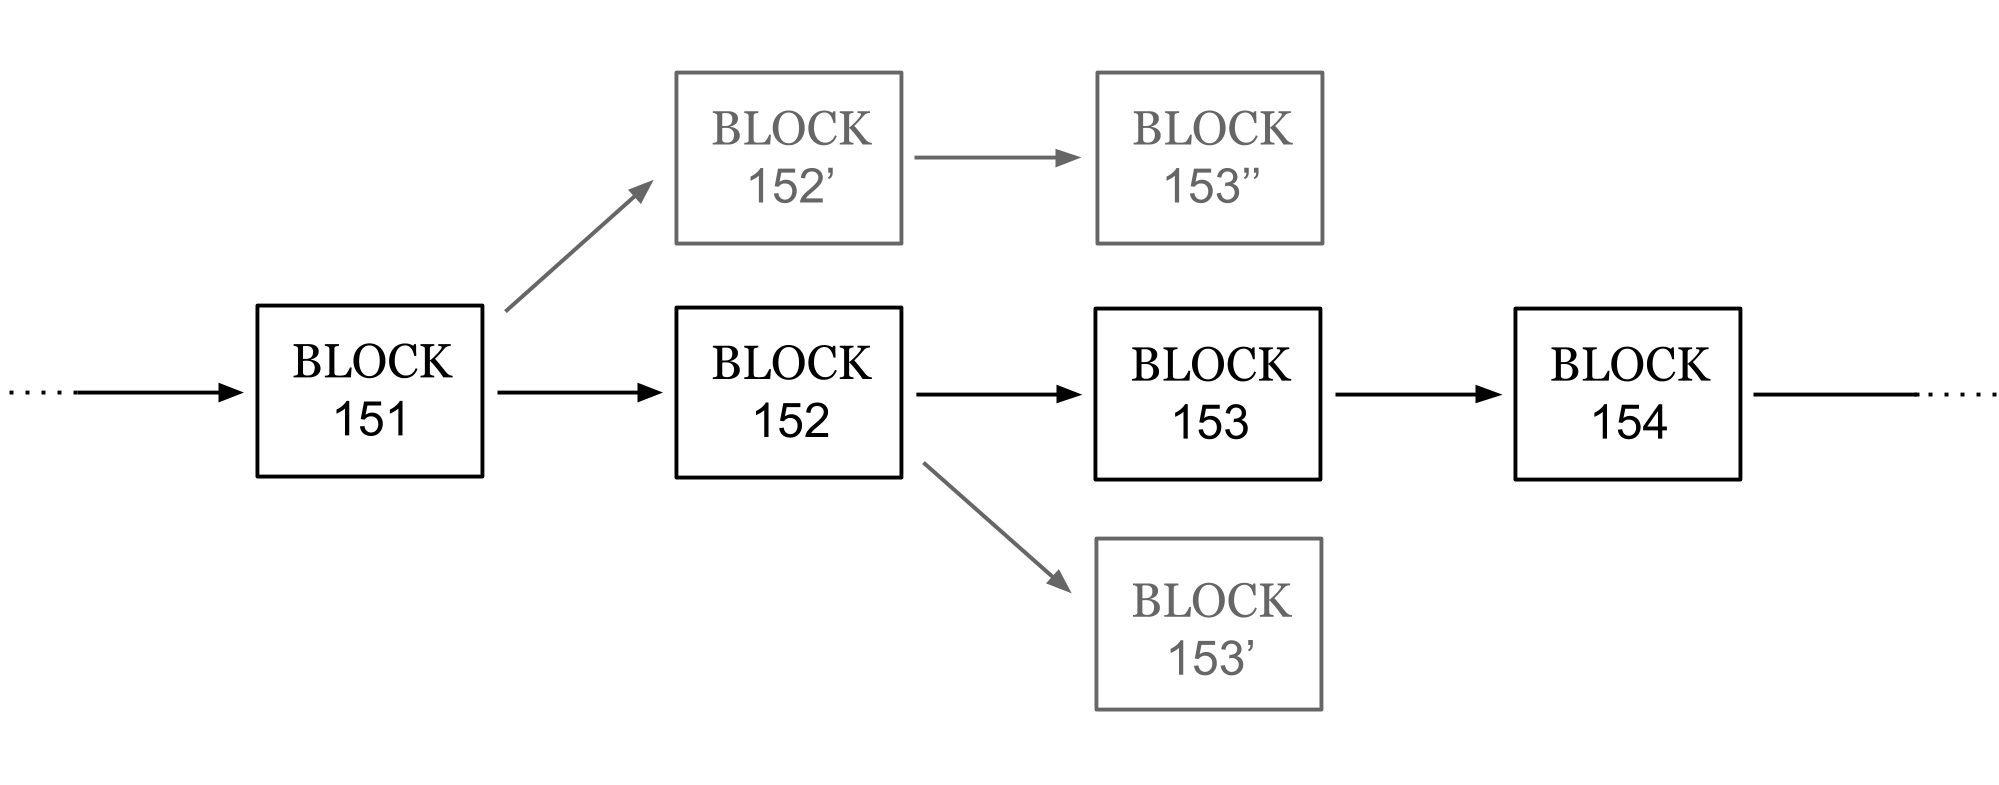
\includegraphics[width=0.9\linewidth]{Images/Diagrams/blockchain_with_pdelay.png}
    \caption{More complex, realistic model of a blockchain (now taking network propagation delay into account). The faded blocks are so-called ``stale''.}
    \label{fig:blockchain_w_pdelay}
\end{figure}

We can calculate the number of stales per found block simply:
\[\textrm{expected\_stale\_rate} = \frac{D}{t_b} \]

We can also calculate the proportion of the blockchain which an attacker would need access to in order to launch a 51\% attack\footnote{Ironically, a so-called 51\% attack does not require an attacker to control $\geq$ 50\% of the total hash-rate. This applies to Ethereum and Bitcoin, though to lesser extent.}. If the attacker is a single node, then the required proportion of network hash power to control the Bitcoin network would be only 49.5\% assuming a network propagation delay $D$ of 12 seconds\footnote{12 seconds\cite{twelve_s_for_btc} is the mean delay to reach 95\% the network for bitcoin.}.
\begin{align*}
    \textrm{proportion\_needed} &= \frac{1-\textrm{stale\_rate}} {2-\textrm{stale\_rate}} \\
    &= \frac{1 - (12 / 600)} {2 - (12 / 600)} \\
    &= \frac{0.98}{1.98} \\
    &\approx 0.494 \\
    &\approx 49.5\%
\end{align*}

This can also be applied to Ethereum's network details. Here we assume that no stales are included in the blockchain (just like Bitcoin). Thus this figure is significantly lower than in reality. Again we take $D$ to be $\approx$ 12 seconds.
\begin{align*}
    \textrm{proportion\_needed} &= \frac{1 - (12 / 15)} {2 - (12 / 15)} \\
    &= \frac{0.2}{1.2} \\
    &\approx 0.167 \\
    &\approx 16.7\%
\end{align*}

Here, we can see that, with a single node, the attacker would need to control 16.7\% of the network's total hash rate. Since pools of miners often control upwards of 30\% of some cryptocurrencies' networks, it would be unacceptable to release Ethereum without the introduction of the inclusion of ``uncle blocks'' to maintain a secure, trustless platform. The Ethereum platform rewards those who have mined uncle blocks or included a reference to uncle block(s) and this provides a secondary incentive to mine the coin. This means that the idea of mining stale blocks doesn't result in fewer miners on the network.





\subsection{Cryptography}
Cryptography in computer science is the subject of analysing and creating codes to encrypt data. This is a very important principal feature of all cryptocurrencies and most blockchains. Without cryptography, Bitcoin, Monero and Bitmessage would not be possible. It is an essential building block of trustless interaction and cannot be ignored.

\begin{figure}[h]
    \centering
    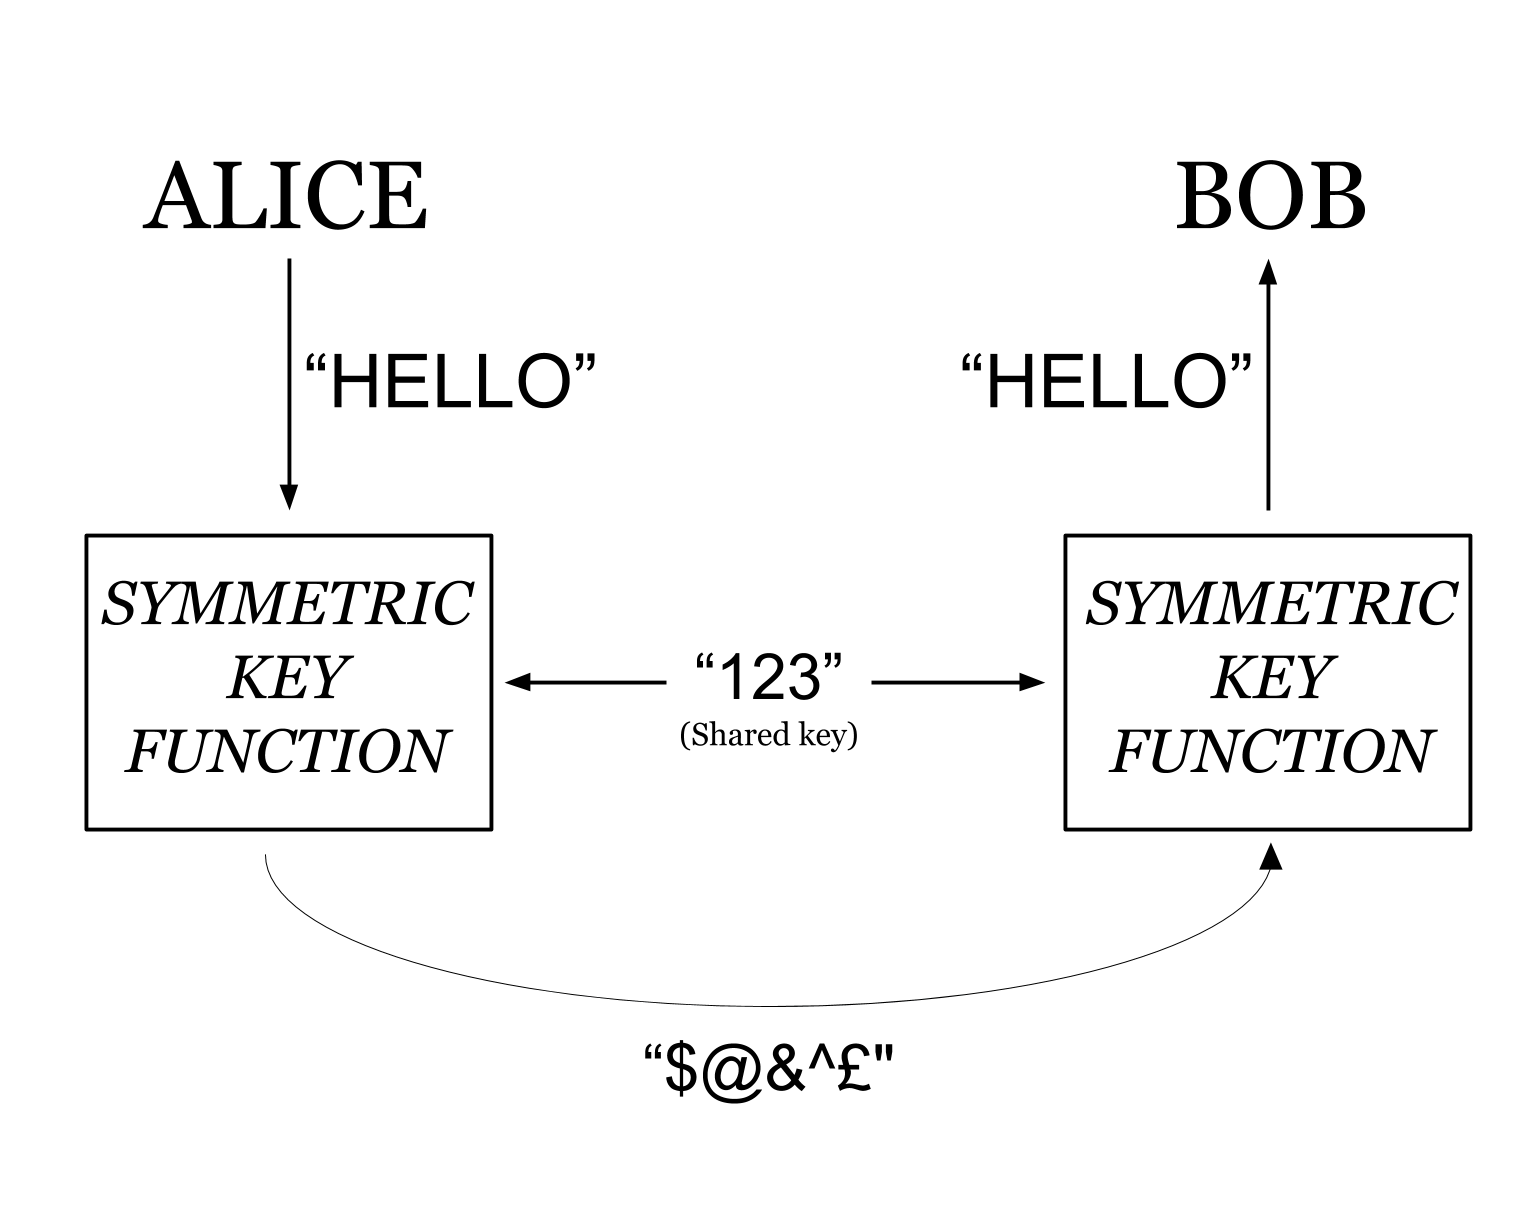
\includegraphics[width=0.5\linewidth]{Images/Diagrams/symmetric_key_encryption.png}
    \caption{Symmetric Key Encryption. Alice encrypts her text with the key 123. The resulting cipher-text is ``\$@\&\textasciicircum£''. Bob decrypts her cipher-text with the key 123. Onlookers are unable to decipher the message without knowledge of this key.}
    \label{fig:symkeyenc}
\end{figure}
\newpage
\subsubsection{Symmetric Key Encryption}
Symmetric key encryption is the encryption and decryption of data with one shared key (see \autoref{fig:symkeyenc}). This key is known only to the creator/sender of the message-data and its intended recipient.
Examples of this form of encryption include AES\cite{aes}, DES and Blowfish. This form of encryption can be very useful for fast encryption and decryption which is ideal for high traffic situations. It is used extensively for internet traffic secured with TLS (Transport Layer Security). However, it used very little in the context of blockchains and cryptocurrencies.

\subsubsection{Hash Functions} \label{subsubsec:hashfns}
Hash Functions are algorithms that (hopefully) irreversibly 'encrypt' data. They take some input and return a pseudo-random string of data (see \autoref{fig:hashfns}). For most hash functions, the length of output is fixed. Hash Functions are intended to provide a unique output for every input though on very rare occasions, this is not the case. Importantly, they always return the same value given the same input. This means that they can be used for checking data integrity. For example, if someone wanted to make sure that a message did not get corrupted in transit, they could attach a 'hash' (output of hash function given message as an input) of the message to the end of the message. The recipient of the message could then use the same hash function to hash their received message. If his calculated hash is the same as the sender's included hash, when compared, then the message data's integrity has been maintained.
\begin{figure}[h]
    \centering
    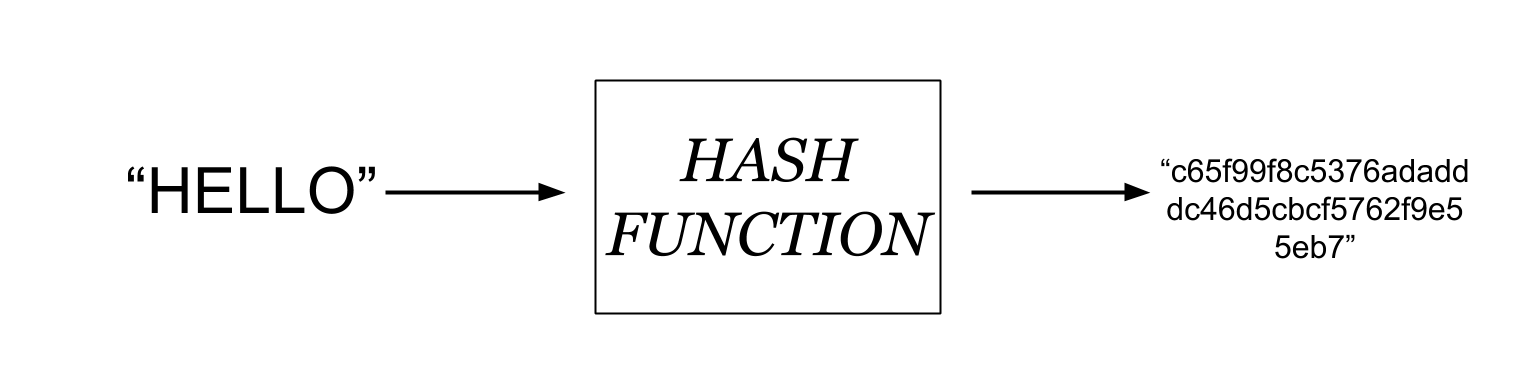
\includegraphics[width=0.8\linewidth]{Images/Diagrams/hash_function.png}
    \caption{Hash Function. In this case the hash function ``SHA-1'' is used to hash the word ``HELLO'' into the following pseudo-random output: ``c65f 99f8 c537 6ada dddc 46d5 cbcf 5762 f9e5 5eb7''}
    \label{fig:hashfns}
\end{figure}

However, it would still be possible for a malicious party to intercept and tamper with a message since they can just recalculate the hash after modifying the message content.

\subsubsection{Asymmetric Key Encryption/Signing}
Asymmetric key encryption is the encryption and decryption of data with two different keys (see \autoref{fig:asymkeyenc}). Typically, one of these keys is known as the public key and the other is known as the private key. The public key is shared around and normally accessible to anyone. The private key is kept secret and is only ever known to the owner of the key. When someone wants to send some data, they encrypt it with the recipient's public key. It is now impossible for anyone to successfully decrypt the cipher-text unless they have access to the recipient's private key. This form of encryption is the method used by Bitmessage to secure messages. 

Whilst it is computationally easy to derive a public key from a private key, it is extremely computationally difficult to do the reverse. This is the basis for asymmetric keys. The mathematical formulae used to derive the keys utilise the intractability of certain fields of mathematics such as the ``Discrete Logarithm Problem'' to allow for this.

\begin{figure}[h]
    \centering
    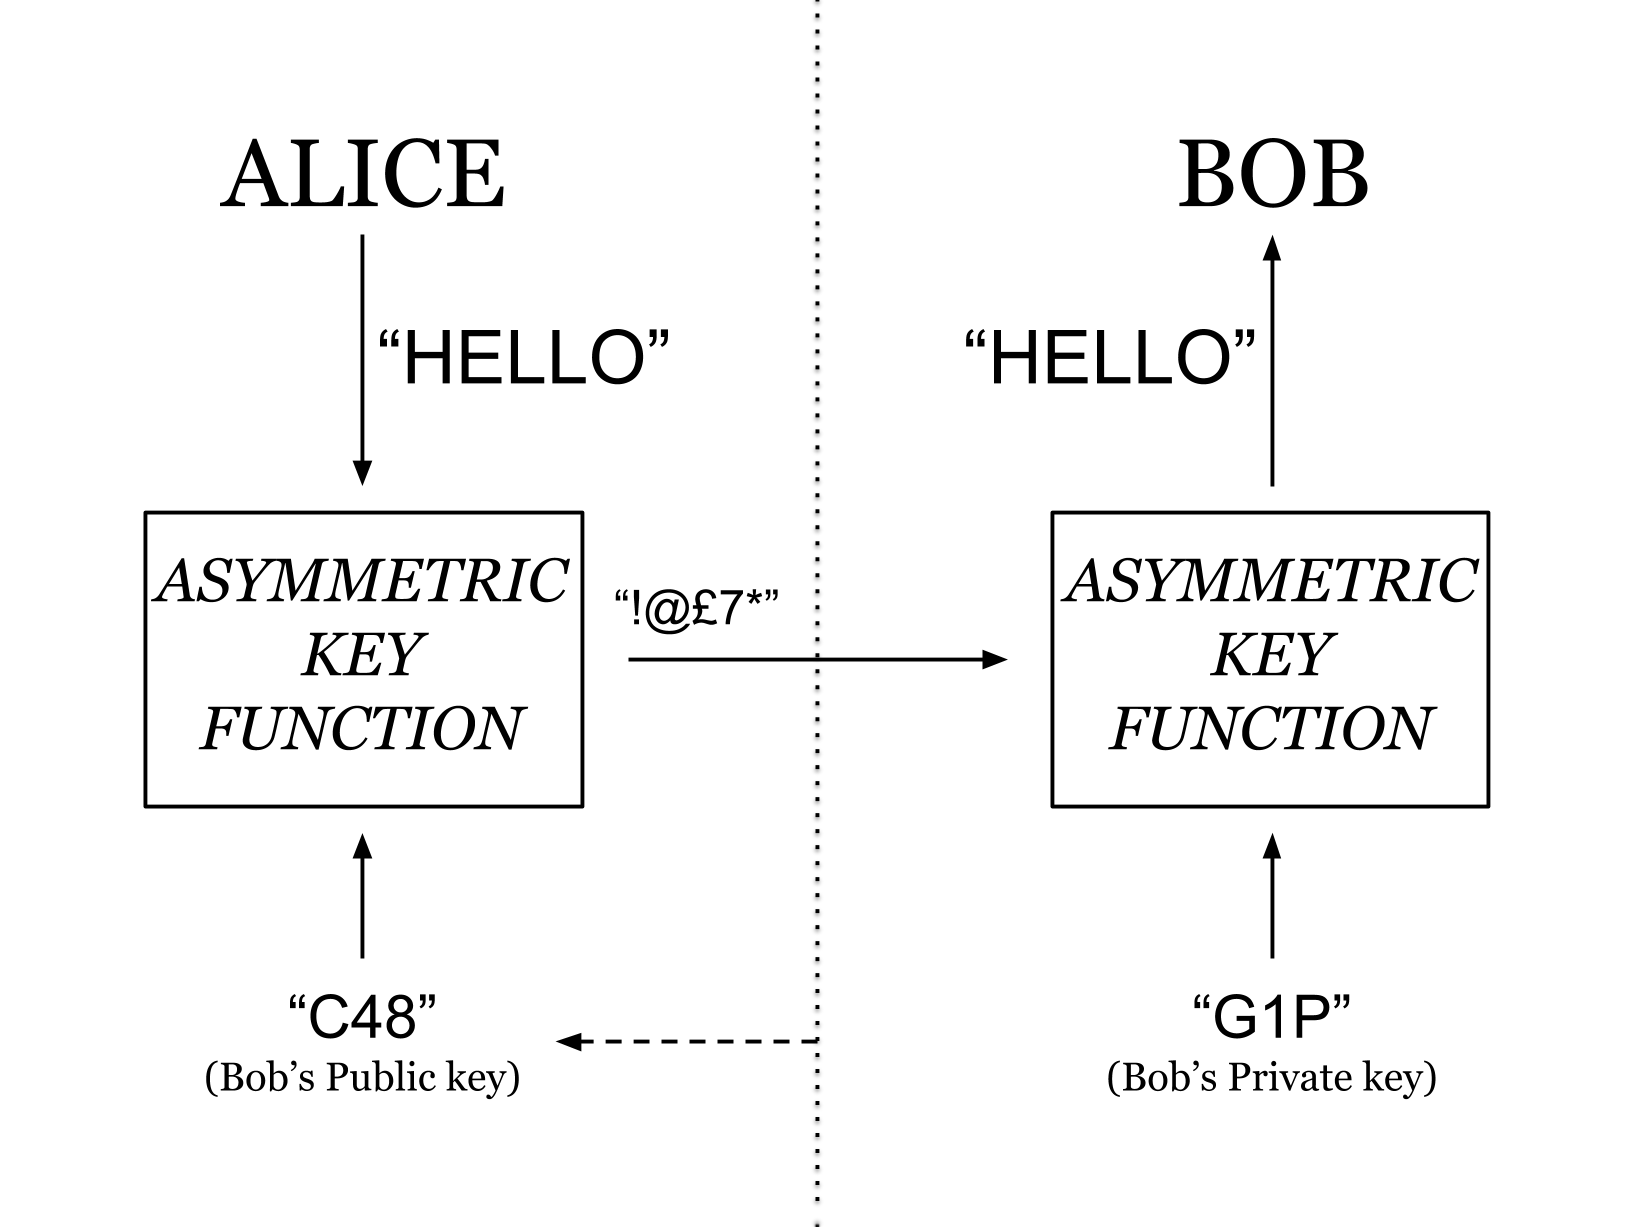
\includegraphics[width=0.6\linewidth]{Images/Diagrams/asymmetric_key_encryption.png}
    \caption{Asymmetric Key Encryption. Alice encrypts her text with Bob's public key C48. The resulting cipher-text is ``!@£7*''. Bob then decrypts Alice's cipher-text with his private key G1P.}
    \label{fig:asymkeyenc}
\end{figure}

Asymmetric key encryption is normally more useful than the symmetric equivalent because it does not require a secret key exchange; No secret information is ever exchanged and therefore there is very little risk of a compromise in security during communication.
Asymmetric key encryption can also be 'reversed' to create Asymmetric key signatures (see \autoref{fig:asymkeysig}). A signed message is created by encrypting some data with the sender's private key. It is then only able to be decrypted by the sender's public key. Since this public key is widely accessible to anyone, these allow anyone to verify the sender of the message. This is useful when someone needs to verify the authenticity of the message but the content of the message is intended for public access (data is not encrypted). This is again used extensively in blockchain applications such as Bitcoin and Monero.

\begin{figure}[h]
    \centering
    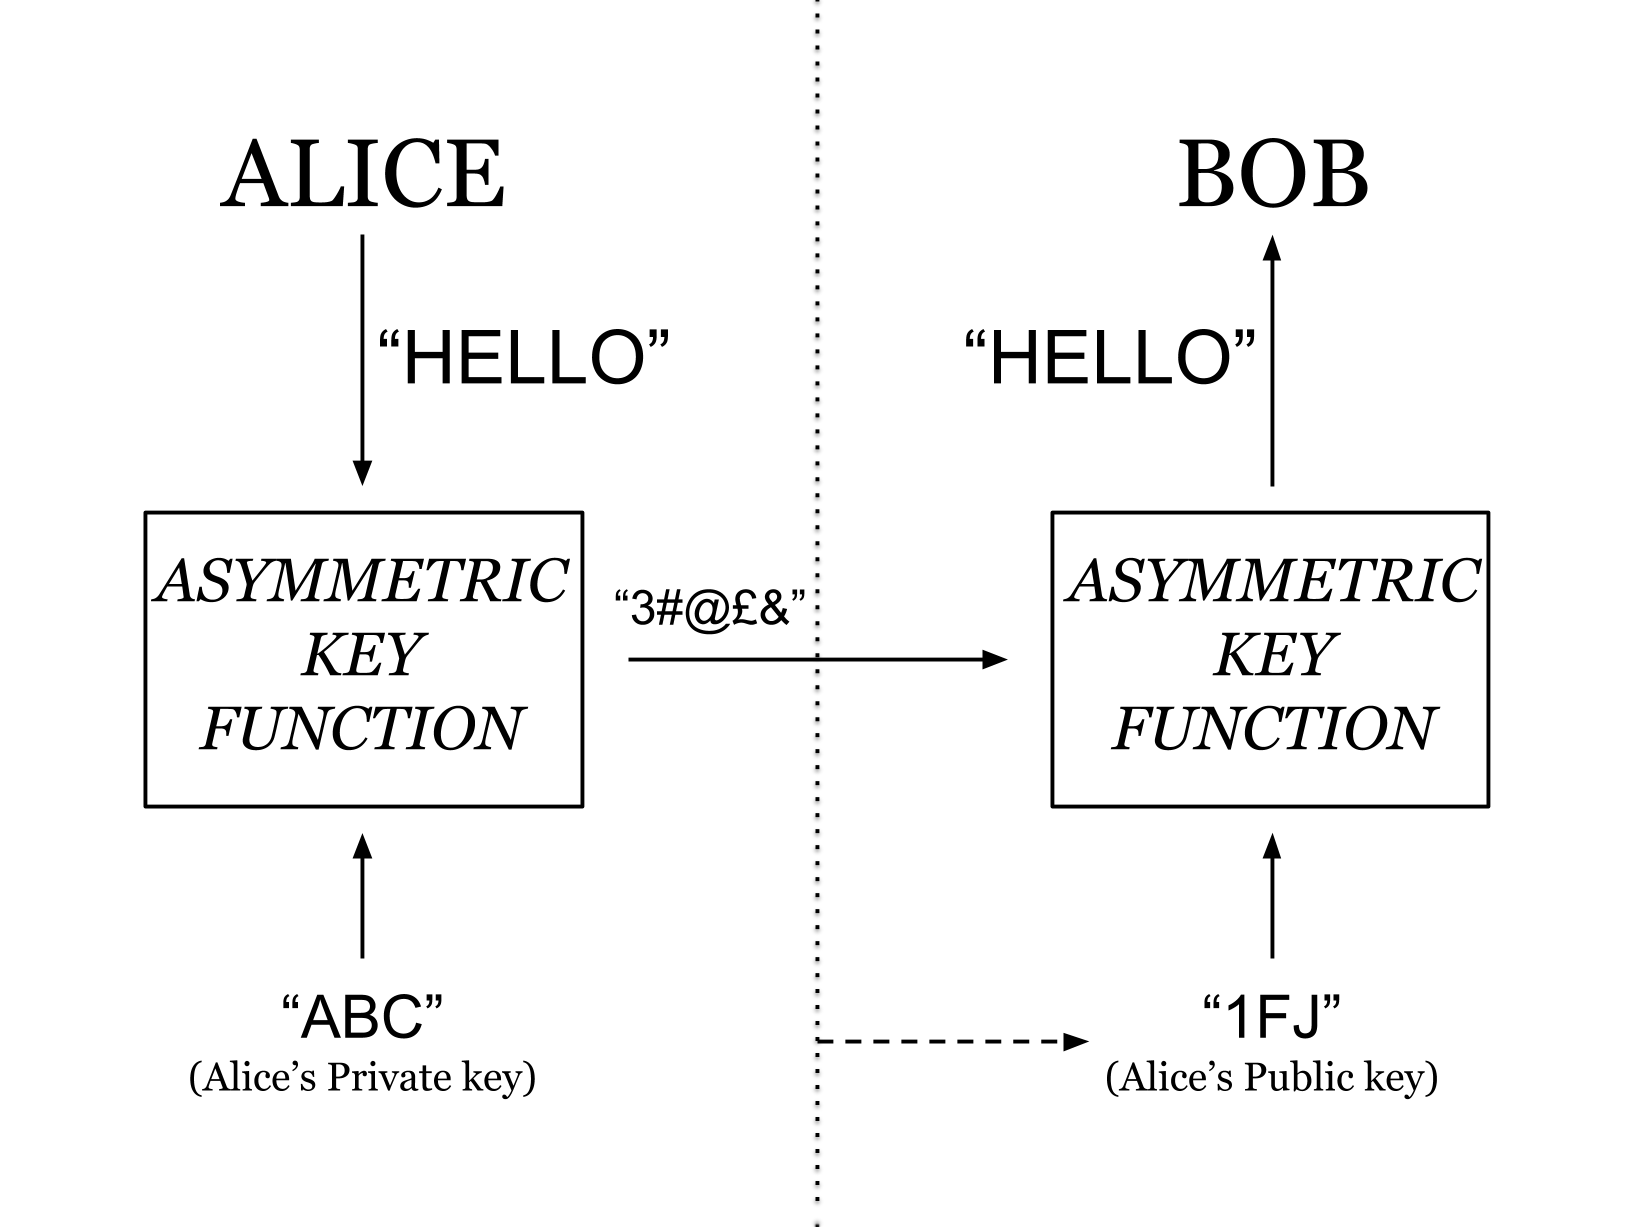
\includegraphics[width=0.6\linewidth]{Images/Diagrams/asymmetric_key_signature.png}
    \caption{Asymmetric Key Signature. Alice encrypts her text with her private key ABC. The resulting cipher-text is ``3\#@£\&''. Bob then decrypts Alice's cipher-text with Alice's public key 1FJ, thereby verifying that Alice is the sender.}
    \label{fig:asymkeysig}
\end{figure}

Examples of Asymmetric key encryption/signature algorithms include RSA, DSA and Elliptic Curve. RSA is an older standard which requires relatively large key sizes to provide a respectable level of security and is therefore not used much in the context of blockchains and cryptocurrencies though is still very popular elsewhere. It relies on the intractability of computing integer factorisation. DSA is a similar standard but only allows for signatures and no encryption or key exchange (DSA relies on the intractability of the Discrete Logarithm Problem).

\subsubsection{Elliptic Curve Cryptography (ECC)}
Elliptic curve cryptography is the encryption system of choice for all contemporary cryptocurrencies. Here\cite{ic_encryption_course} is a useful guide that I found during research that explains modular arithmetic and finite fields well. It is public/private-key based and relies on the computational difficulty of the Elliptic Curve Discrete Logarithm Problem.

\paragraph{Modular Arithmetic}
Modular Arithmetic is used in many asymmetric encryption systems. The idea of modular arithmetic is to work with remainders of divisions. For example: \[9 \equiv 1\ (\textrm{mod}\ 4),\]\[3 \equiv 3\ (\textrm{mod}\ 9)\]{\centering and \par}\[18 \equiv 0\ (\textrm{mod}\ 9)\]

The number 9 is congruent to 1 in (mod 4) space since 9/4 gives remainder 1. Likewise 3 is congruent to 3 in (mod 9) space since 3/9 gives remainder 3. 18 is congruent to 0 in (mod 9) space since 18/9 gives remainder 0. Any integer $r\ (\textrm{mod}\ m)$ can be written as $k*m+r,\ k \in \mathbb{Z}, r \in \mathbb{N}$. Note that, here, $0 \in \mathbb{N}$.

However, one must be careful with negative numbers since although $9 \equiv 1\ (\textrm{mod}\ 4)$, $-9 \not\equiv 1\ (\textrm{mod}\ 4)$. This is because $9=2\times4+1$ but $-9\not=-2\times4+1$. In fact, $-9=-3\times4+3$. Therefore $-9 \equiv 3\ (\textrm{mod}\ 4)$.

Modular arithmetic can also be thought of as a clock face. When the 'hours hand' passes through twelve it resets back to one as if the time is constantly being divided by 12 and remainder taken. Modular arithmetic is sometimes also known as 'Clock Arithmetic' for this reason.

Performing simple arithmetic operations to numbers in mod space is quite simple. For example, for addition: \[10+2 \equiv 12 \equiv 4\ (\textrm{mod}\ 8)\]This also applies for subtraction: \[10-2 \equiv 8 \equiv 0\ (\textrm{mod}\ 8)\] Multiplication is just as easy: \[10\times 2 \equiv 20 \equiv 4\ (\textrm{mod}\ 8)\]
However, calculating the division of two numbers in mod space is more complex. Division is not defined for every number and division is only allowed to take place if the divisor has a multiplicative inverse (explained well here\cite{ic_encryption_course}, under the modular arithmetic section).

\paragraph{Finite Fields}
To understand how ECC works, it is important to understand finite fields. Finite fields are also explained well here\cite{ic_encryption_course}. A finite field is a group of numbers (with finite length) containing all integers mod $p$ where $p$ is usually a prime number (in this case it \emph{is} prime). The numbers in the field possess some useful properties:\\
\\Closure:
\[a+b \equiv c\ (\textrm{mod}\ n),\ 0 \leq c \leq n-1\]
Associativity:
\[a\times (b + c) \equiv a\times b + a\times c\ (\textrm{mod}\ n),\ \textrm{for all}\ a,b,c \in \textrm{Field}\]
Contain an Identity element (for $+$ and $\times$):
\[a+0 \equiv 0+a \equiv a\ (\textrm{mod}\ n)\]
\[a\times 1 \equiv 1\times a \equiv a\ (\textrm{mod}\ n)\]

\paragraph{Elliptic Curves}
Elliptic curves are defined as the set of points satisfying the equation $y^2 = x^3+ax+b$ where $4a^3 + 27b^2 \not= 0$ (limited to avoid singular curves). A useful guide that I found on elliptic curve cryptography can be found here\cite{ec_guide}. For cryptography, the curve is defined over a finite, prime field. A single operation is defined for an elliptic curve ($+$). The identity element of the finite field is defined as the point at infinity (written as 0/zero). Here, we are given two points on the curve and are looking for the third (the point that lies on the same line as the other two points as well as the same elliptic curve). If $P,Q,R$ are all defined to be on a line and on the elliptic curve, then the $+$ operation is defined as $P+Q+R=0$. In other words the operation which defines addition in this field takes two points $P,\ Q$ and gives the result $-R$. This is equivalent to finding the mentioned third point and inverting/reflecting it across the x-axis. 
\begin{figure}[h]
    \centering
    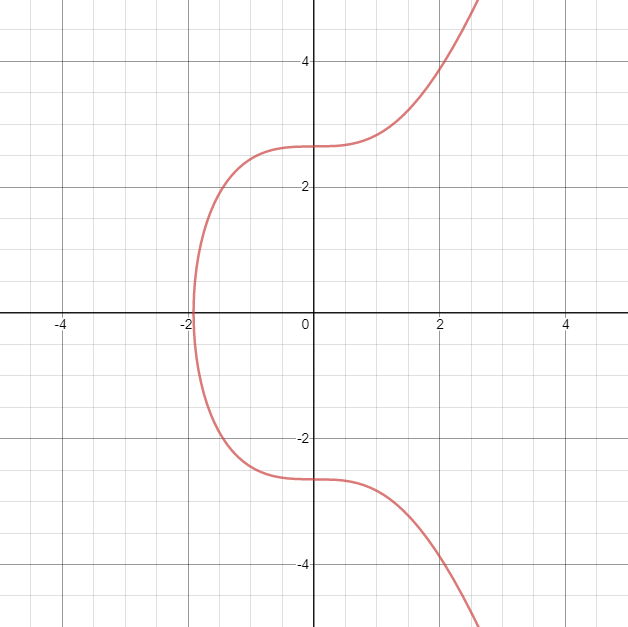
\includegraphics[width=0.5\linewidth]{Images/Secp256k1.png}
    \caption{Elliptic curve secp256k1 $(y^2=x^3+7,\ [a=0,\ b=7])$ over the real numbers. This is the curve used by Bitcoin. Note that when defined over finite field, this would actually look like many scattered points.}
    \label{fig:secp256k1}
\end{figure}

Addition that is repeated many times is said to be the scalar multiplication operation. For example: $nP = P+P+P+P+...+P$, $nP$ is the same as $P$ added to itself $n$ times.
In terms of actually finding the third point on the curve $R=(x_R,\ y_R)$, some algebra can be used:
\[x_R=m^2-x_P-x_Q\ (\textrm{mod}\ p)\]
\[y_R=y_P+m(x_R-x_P)\ (\textrm{mod}\ p)\]
\[\ \ \ \ =y_P+m(x_R-x_Q)\ (\textrm{mod}\ p)\]

If $P\not=Q$:
\[m = (y_P-y_Q)(x_P-x_Q)^{-1}\ (\textrm{mod}\ p)\]

If $P=Q$:
\[m = (3x_P^2 + a)(2y_P)^{-1}\ (\textrm{mod}\ p)\]

In fact, the points that we will use will not all be integers $\leq p$ (where $p$ is prime). This is because, if you take a base-point $G$, then the points $G, 2G, 3G, 4G, 5G... nG$ will form a cyclic subgroup. This means that for example (arbitrary curve parameters) $[G, 2G, 3G]=[4G, 5G, 6G]$. This subgroup will always include zero (the identity element) and so the ``order'' of a base-point is understood to be the number of elements between a base-point and 0. For example, for a base-point $G$, the order of $G$ is the smallest positive integer $n$ for which $nG = 0\ (\textrm{mod}\ p)$. The cofactor $h$ of the subgroup is defined as $N/n$ where $N$ is the order of the elliptic curve and $n$ is the order of the subgroup. $h$ is always an integer since $N$ is a multiple of $n$. This gives us $NP=0$ and therefore $n(hP)=0$. Generally, for cryptography, the base-point is chosen to have a large, prime order.

This gives us 6 parameters for our elliptic curve cryptography algorithm: prime number $p$ (size of finite field), $a$ and $b$ (coefficients in elliptic curve equation), $G$ (a base point that determines the cyclic subgroup), $n$ (the order of the subgroup's order), $h$ (cofactor of subgroup). Sometimes another parameter $S$ is included, this is the seed that can be used to verify that the coefficients $a$ and $b$ are random.

From here we can create a public/private key encryption algorithm. We take the private key to be an integer $d, d \in [1,n-1]$, where $n$ is the subgroup order. We take the public key to be the point $H$ where $H=dG$ and $G$ is the subgroup base-point. This whole algorithm is based around the Discrete Logarithm Problem (it is hard to get $x$ given $P=xQ$ where $P,Q$ are points on the curve).

\paragraph{ECDSA}
ECDSA (Elliptic Curve Digital Signature Algorithm) is the elliptic curve equivalent of the DSA algorithm. It entails taking the hash of some data with a cryptographically-secure hash function. Then signing the hash of the data with the sender's private key. This can then be used as a signature to the message and anyone can verify the authenticity of the message using the sender's public key. This is the signature algorithm used by Bitcoin and most other cryptocurrencies.

\paragraph{Shor's Algorithm}
Although it is computationally intractable for classical computers to compute a private key from a public key, Shor's algorithm reduces the intractability significantly ($\mathcal O(\textrm{log} n)^3$ time complexity) by the use of quantum computers. However, the contemporary quantum computers are not capable of such calculations yet.

\subsection{Messaging Platform Features}
During research, I looked through all the messaging apps that I considered popular, looking for desirable features that would improve the user experience on a messaging platform. I have devised the following list of features that I would like to be made available:
\begin{itemize}
    \item Group Chats
    \item Stickers
    \item Message Receipt Acknowledgements
    \item Message Reactions
    \item QR Code Addresses
\end{itemize}

\subsubsection{Group Chats}
Group chats are a staple feature of all current, major messaging platforms including Facebook Messenger and Whatsapp. Group chats are chats with multiple people on them rather than just two. However this could be hard to design for and could lead to weaknesses in the security of the platform.

In Bitmessage, the closest thing to a group chat is a ``chan'' or channel. Users subscribe to channel addresses which are just addresses controlled by multiple people. This is the equivalent of an email mailing list (except the recipients decide whether they are on the list rather than the sender).

To implement group chats into my proposed platform, I think I would have a private key for the chat which is shared to all users in the group when created. Each user in the group would use this private ``view'' key to see the contents of the message (similar to Monero's ``view'' and ``spend'' key). They could then use a separate, private ``send'' key to allow them to send messages to the group. Each message to the chat would be required to include a signature (signed with sender's own private ``send'' key) so that the sender of the message can always be determined by others in the group.

\subsubsection{Stickers}
Stickers are a modern modification to typical messaging apps. They are similar to emojis in that they are images as opposed to plain-text. In my opinion, this is best implemented in Apple's iMessage. Stickers are often animated providing a more entertaining and interesting way of chatting with friends. This should be relatively easy to implement as they are just another form of message.

\subsubsection{Message Receipt Acknowledgements}
Older messaging platforms including SMS fail to show a user when their sent message has been received. Again, I think that this is a very important feature as it is very useful to know if your message has been seen. This will be relatively easy to design for but it will be hard to make the feature compulsory (ie. every user has to acknowledge that they have received a message).

\subsubsection{Message Reactions}
Since I have started using Facebook Messenger, I have really enjoyed using the message reaction feature and I think that it adds a lot to the user experience of the platform allowing for more interesting communication. This feature allows the user to 'react' to a message on a chat with a small animated emoji (usually laughing or crying). It would also be important to include the ability to reply to messages with more messages. This could be quite easy to design for since, again, it is just another form of message.

\subsubsection{QR Code Adresses}
Although perhaps underused, Snapchat has a feature known as Snapcodes that allow a friend to quickly add them as a friend. All they have to do is scan the code and the app does all the work. This would be an important feature of the proposed platform since addresses will probably be unwieldy and hard to remember (long strings of random characters). This should be fairly easy to design for since it is easy to convert a string of characters into a QR code.


\subsubsection{Minimising Storage/Computation for Clients}
It will be important to manage client resource requirements carefully (for example, client devices like mobile phones should not need to store 120GB of blockchain all the time as this is impractical and would be unpopular). To address the problem of limited client storage resources, I have researched into the feasibility of the following solution. All ``semi-thin'' clients (typically anyone's smartphone who has the app) will only store a random portion of the blockchain. This random portion will be small but with enough devices on the network, this should mean that no blocks are lost from the network entirely. All ``full-node'' clients will store the entire blockchain all the way from the genesis block. However, I do not expect there to be a huge excess of ``full-nodes'' as they will be expensive to maintain with no incentive except the good of the network.
''Semi-full-nodes'' will store all blocks back to a certain expiry date (similar to Bitmessage). These clients could also prune of all messages that have been acknowledged as received (this takes inspiration from Monero's blockchain pruning system \cite{monero_pruning}. All this together would mean that it should be very easy for a ``thinner'' client to access very recent messages, but progressively harder to retrieve older messages. However, importantly, all messages that were ever sent, will always be eventually retrievable and never completely lost from the network. This differs from Bitmessage's system where all messages are eventually deleted from message-pools.

It will also be important to keep computation minimal for client devices. For this reason, the client software could be made to only ``mine'' on the network when the application is open in use, once the use of the network has become sufficiently large and stable. This would provide a fairly constant supply of computational power to compute hashes for blocks (mining). A cryptographic hashing algorithm which favours mobile devices and desktop computers would have to be chosen so as not to allow a single group of high-power servers to single-handedly perform a so-called 51\% attack\cite{51_attack}. Also, I have researched into finding a method to prevent scanning of the blockchain (in the manner of Bitmessage) as this would take up significant computational power on the client or node or both as well as network traffic. Bloom filters are a useful cryptographic tool to help bypass this floor so I may decide to use this.

\subsubsection{Scalability}
Peer-to-peer networks are inherently unstable in their early stages. This is because there are fewer nodes on the network meaning that at some points, not only could the network go down but data could be lost. It would also be easy for a malicious party to perform a so-called 51\% attack where someone controls the majority of the computational-power on the network and can begin to falsely create their own blocks. It would be easier for an attacker to exploit this on a messaging platform since their is no incentive to mine in the first place so it can be expected that many fewer nodes will mine and therefore the total computation (``hash-rate'') of the network will be lower than that of Bitcoin, for example, even with the same number of active users.

\subsection{Ethics}
Whilst proposing the project to various friends and family, I was repeatedly questioned on the topic of ethics. ``Is it ethical to design a platform that could be used by paedophiles, serial-killers and drug-dealers to aid their business?'' My opinion is that the ability to communicate privately is a basic requirement for a society and the people in it. I believe that this is a form of free-speech and regardless of who uses it, it should be protected. However, to clarify, I do not encourage or endorse criminal acts in any way.

In any respect, the secure messaging platforms (Whatsapp, signal etc.) of today could be asked the same questions supposing that they are indeed secure and not monitored. Indeed, many people believe that they do monitor users' messages\cite{whatsapp_endtoend}\cite{facebook_nsa}\cite{fbmsg_nsa_criminal}.

The aim of this project is to bring truly secure messaging to the world, allowing those whose free speech is limited by their political or social circumstances to communicate freely and effectively. In some oppressive regimes, individuals can be subject to imprisonment or other punishment if they speak up against their leaders or governments. This, in my opinion, is simply not fair and everyone deserves the right to say what they want for the good of others. I certainly don't believe in the censorship or monitoring of users' communications and I think that many would agree that the right to privacy is very important.

Data-ownership is another key issue in the contemporary world of the internet and online business. Advertisement has become an unbelievably powerful force, potentially swaying election results across the world as well as allowing large businesses to target new customers. The ``backbone'' of advertisement is the collection and hoarding of user-data. Data is collected, absorbed and sold by businesses online sometimes not only without the users' knowledge but also without their express consent. On top of this, many of the popular services which we use today will simply refuse to function without the consent of the user to give away their data rendering them unusable. This project targets this growing issue and attempts to fix it by entirely eliminating the centralised nature of a messaging service. There is no hidden incentive to create this service and the inability to collect user data is inherent to the design of it. This project is not to make money but to improve real people's lives and that is fundamental to its design. 

\subsection{Conclusion to Research}
I have successfully researched into all the topics that I had planned to and I now feel confident to begin the design/development section of the project. I feel that I have now achieved the understanding which I desired at the beginning of the project and am now suitably knowledgeable to begin theorising a solution.

\newpage

%%%%%%%%%%%%%%%%%%%%%%%%%%%%%%%%% DESIGN %%%%%%%%%%%%%%%%%%%%%%%%%%%%%%%%%

\section{Design}

\subsection{General}
Whilst theorising a solution, I realised that it would be sensible to categorise the different designs into sections to make the whole process easier to manage. I decided to split the bulk of the project into the design of the blockchain itself; the network protocol; and finally the client software.

\subsection{Blockchain Architecture}
This section describes the design process for all elements of the blockchain. It works from the smallest element (a single message transaction) up to the block structure itself and the database structure.

\subsubsection{Transactions}
Message transactions\footnote{Although I will refer to these as transactions, they will not be monetary exchanges. The word ``transaction'' is used for simplicity as it is the term used by nearly all other blockchain projects (mainly cryptocurrencies).} (tx) would be the smallest elements in the proposed Blockchain. As a starting-point, I decided to use the Bitcoin implementation of a tx\cite{bitcoin_protocol}. This had the following structure:

\begin{table}[H]
\centering
\begin{tabular}{ |l|p{8.5cm}| }
\hline
\rowcolor{tblgrey}
Description   & Comments                                                                   \\ \hline
version       & Transaction data format version (note, this is signed).                    \\ \hline
flag          & If present, always 0001, and indicates the presence of witness data.       \\ \hline
tx\_in count  & Number of transaction inputs (never zero).                                 \\ \hline
tx\_in        & A list of 1 or more transaction inputs or sources for coins.               \\ \hline
tx\_out count & Number of transaction outputs.                                             \\ \hline
tx\_out       & A list of 1 or more transaction outputs or destinations for coins.         \\ \hline
tx\_witnesses & A list of witnesses, one for each input; omitted if \textit{flag} is omitted above. \\ \hline
lock\_time    & The block number or timestamp at which this transaction is unlocked.       \\ \hline
\end{tabular}
\end{table}

I then began to strip away the features that were not necessary for this project. These mainly included:
\paragraph{Multiple Inputs/Outputs}
Bitcoin and all other cryptocurrencies split inputs and outputs into many different pieces (See \autoref{fig:bitcoin_many_in_out}). This is how fractions of coins can be exchanged (otherwise the currency would become unwieldy). This does not make sense for a messaging platform and is therefore not reasonable to implement. This can therefore be discarded for the next iteration of my tx design.
\begin{figure}[h]
    \centering
    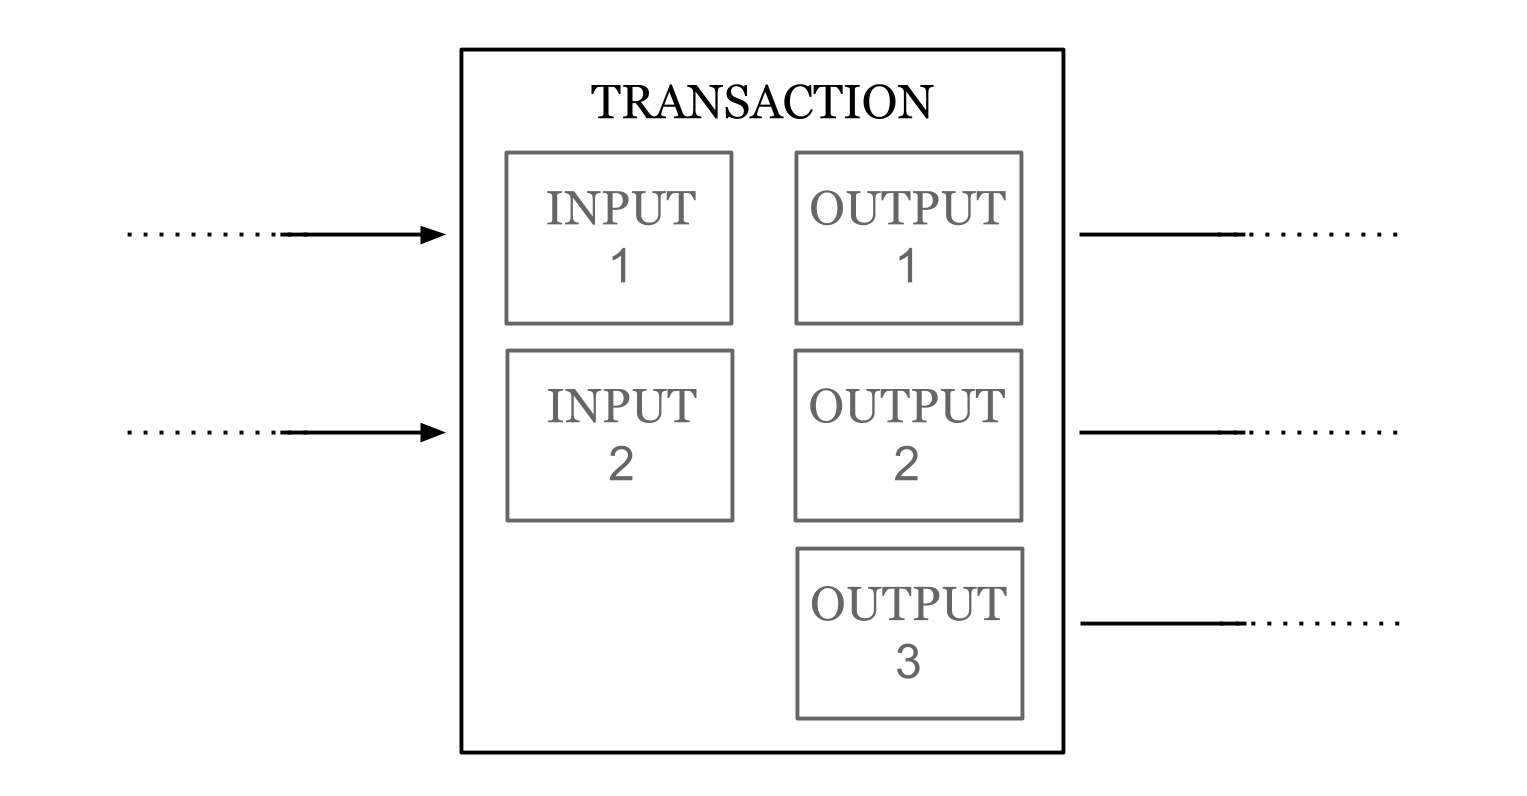
\includegraphics[width=0.75\linewidth]{Images/Diagrams/blockchain_many_inputs_outputs.png}
    \caption{Each transaction in a cryptocurrency contains one or many inputs and one or many outputs (with the exception of ``Coinbase'' transactions where new coins are created).}
    \label{fig:bitcoin_many_in_out}
\end{figure}

\paragraph{Witness Data}
Witness Data was first introduced to Bitcoin in 2015 with SegWit\cite{bitcoin_segwit}. It allows 'thin' clients to verify transactions without possessing a large proportion of the blockchain whilst fixing transaction malleability problems. This might seem like it would be especially useful for my project since the issue of client storage/computing resource management is very important. However, the method that SegWit uses to verify transactions is specific to cryptocurrencies and is therefore not exactly applicable. For example, Bitcoin's transactions contain a list of past transactions as inputs that are a by-product of dealing with money (as mentioned above). Validation is much easier for a messaging platform since a simple signature (and potentially a proof-of-work) is enough to verify the authenticity and validity of a message.
\begin{figure}[ht]
    \centering
    
\includegraphics[width=0.65\linewidth]{Images/Segwit.png}
    \caption{Bitcoin's SegWit has allowed for new innovations in the Bitcoin network such as the \textit{Lightning Network}\cite{bitcoin_lightning_network} whilst maintaining backward compatibility.}
    \label{fig:segwit}
\end{figure}
\newpage

Having stripped the above features from the structure of a transaction, I now have a simplified model:
\begin{table}[H]
\centering
\begin{tabular}{|l|p{8.5cm}|}
\hline
\rowcolor{tblgrey}
Description & Comments                                                  \\ \hline
version     & Transaction data format version (note, this is signed).   \\ \hline
tx\_from    & Address of sender (0x0 for anonymous).                    \\ \hline
tx\_to      & Address of recipient.                                     \\ \hline
tx\_sig     & Cryptographic signature of transaction.                   \\ \hline
lock\_time  & The block number or timestamp at which this transaction is unlocked. \\ \hline
\end{tabular}
\end{table}

\paragraph{Enabling Group Chats}
To allow for group chats, I needed a way to distribute messages to many people. One solution for this would be to have the sender send a separate message to each member of the group (One to Many). However, this is obviously a bad idea as it will require $n$ transactions for the same message.

Another solution fixes this problem by having a distributed private key for the group (ie.\ the group has its own address and every user in the group possesses the private  and public keys; One to One). This means that when a user wants to join a new group chat, they do not have to be added to everyone's individual table of recipients. Bitmessage uses a One to One system with a similar structure.

\newpage

\textbf{One to Many}
\textit{ - Advantages}
\begin{itemize}
    \item Everyone knows exactly who is in the group.
    \item Messages can be sent to the group but exclude selected people (effectively allowing users to ``kick'' others from the group).
\end{itemize}

\textit{ - Disadvantages}
\begin{itemize}
    \item Pollutes network and blockchain with the same repeated message. (Alternative is to complicate messages with multiple outputs)
    \item Computationally intensive to generate proof of work for every transaction.
    \item Database of users in group has to be propagated through all users in the group every time someone wants to join.
\end{itemize}


\textbf{One to One}
\textit{ - Advantages}
\begin{itemize}
    \item One transaction per message. (maintaining network and blockchain health)
    \item New users can be added easily.
    \item Tried and tested by Bitmessage. Strong solution.
    \item Doubles as a broadcast channel system for subscription-style update-feed. (Bitmessage ``chans'')
\end{itemize}

\textit{ - Disadvantages}
\begin{itemize}
    \item If someone has access to the private key, then they can eavesdrop on conversations without being known. (applies to normal message conversations anyway)
    \item Transactions require some ``post-processing'' from clients. (treat as group chat instead of two-user conversations)
\end{itemize}

From the above information, it should be clear to see that the best solution is One-to-One. Therefore this is the solution that I will carry forward.
\newpage

\paragraph{Stickers and Message Types}
If I want to allow for the functionality of a modern messaging service, then I will need to have different kinds of messages. For example, if I want 'stickers' to be available, then it would make sense to have that as a message-type. I have compiled all the message types into the following table:
\begin{table}[H]
\centering
\begin{tabular}{|p{3cm}|p{8.5cm}|}
\hline
\rowcolor{tblgrey} 
Message type    & Description                                                                               \\ \hline
text            & Simple message in text. (default)                                                         \\ \hline
acknowledgement & A message that contains no actual content, only to indicate that a message has been read. \\ \hline
sticker         & Contains a type of sticker and a position for it in the chat.                                        \\ \hline
reaction        & Similar to Acknowledgement but contains either a Unicode character (emoji) as a reaction or a text reply. \\ \hline
file            & Similar to text but is binary file contents instead of plain text.                       \\ \hline
\end{tabular}
\end{table}

Through the above list of message-types, users should be able to communicate effectively and expressively in a similar manner to that of Facebook Messenger or Whatsapp. For each of these message types, I have decided what fields should be set.

If a user chooses to create a simple `\textbf{text}' message, then the following fields should be set.
\begin{table}[H]
\centering
\begin{tabular}{|p{2.5cm}|p{8.5cm}|}
\hline
\rowcolor{tblgrey} 
Field           & Description                                               \\ \hline
encoding        & Encoding standard for decoding bytes to text. (eg. UTF-8) \\ \hline
data            & Simple plain-text message.                                \\ \hline
\end{tabular}
\end{table}

If a user chooses to create an `\textbf{acknowledgment}' message, then the following field should be set.
\begin{table}[H]
\centering
\begin{tabular}{|p{2.5cm}|p{8.5cm}|}
\hline
\rowcolor{tblgrey} 
Field           & Description                                               \\ \hline
msg\_id         & The msg\_id of the message which is being acknowledged.   \\ \hline
\end{tabular}
\end{table}

If a user chooses to create a `\textbf{sticker}' message, then the following fields should be set.
\begin{table}[H]
\centering
\begin{tabular}{|p{2.5cm}|p{8.5cm}|}
\hline
\rowcolor{tblgrey} 
Field           & Description                                               \\ \hline
sticker\_pack   & The sticker pack which contains the chosen sticker.       \\ \hline
sticker\_index  & The index of the chosen sticker in its sticker pack.      \\ \hline
\end{tabular}
\end{table}

If a user chooses to create a `\textbf{reaction}' message, then the following fields should be set.
\begin{table}[H]
\centering
\begin{tabular}{|p{2.5cm}|p{8.5cm}|}
\hline
\rowcolor{tblgrey} 
Field           & Description                                               \\ \hline
msg\_id         & The message to be responded to.                           \\ \hline
encoding        & Encoding standard for decoding bytes to text.      \\ \hline
data            & Plain-text message data (could be single Unicode character or string reply).      \\ \hline
\end{tabular}
\end{table}

If a user chooses to create a `\textbf{file}' message, then the following fields should be set.
\begin{table}[H]
\centering
\begin{tabular}{|p{2.5cm}|p{8.5cm}|}
\hline
\rowcolor{tblgrey} 
Field           & Description                                               \\ \hline
file\_name      & Name of file.                                             \\ \hline
file\_type      & Type of file (eg. PDF, PNG, JPEG).                        \\ \hline
data            & Binary file data.                                         \\ \hline
\end{tabular}
\end{table}

\textit{TODO: v2 make array of files instead of just one file}

You will notice that a new field now has to be introduced to a message transaction in order for \textbf{acknowledgment}s and \textbf{reaction}s to work. I call this the \textbf{msg\_id} and this provides a way of referencing an previous message\footnote{It could also serve as the primary key for messages in a client's message database when messages need to serialised to disk.}.

Now that I have a new field, I will add that to the list of tx fields. Now a transaction looks as follows. Here I also add in the fields for message type and message data.
\begin{table}[H]
\centering
\begin{tabular}{|p{2.5cm}|p{8.5cm}|}
\hline
\rowcolor{tblgrey}
Description & Comments              \\ \hline
version     & Transaction data format version.                              \\ \hline
lock\_time  & The block number or timestamp at which this transaction is unlocked. \\ \hline
tx\_from    & Address of sender (0x0 for anonymous).                        \\ \hline
tx\_to      & Address of recipient.                                         \\ \hline
tx\_sig     & Cryptographic signature of transaction.                       \\ \hline
msg\_id     & msg\_id of message. (used for acknowledgements and reactions) \\ \hline
msg\_type    & Type of message. (text, acknowledgment, sticker...)          \\ \hline
msg         & Message object. (has different subfields depending on msg\_type, as above) \\ \hline
\end{tabular}
\end{table}

\textit{TODO: v2 add tx\_id for eliminating duplicates from entering blocks.}

\newpage
\label{para:bf}
\paragraph{Bloom Filters}
A good way of improving search efficiency in the blockchain would be to implement Bloom filters. Bloom filters give an indication as to whether or not a particular item is in a data set. They are probabilistic data structures meaning that they indicate either that an item \textit{may} be in a set or that it is \textit{definitely not} in a set. This is obviously very helpful as it would mean far fewer blocks would have to be transmitted through the network and clients would no longer have to intensively search through every single block when searching for any incoming messages.
\begin{figure}[h]
    \centering
    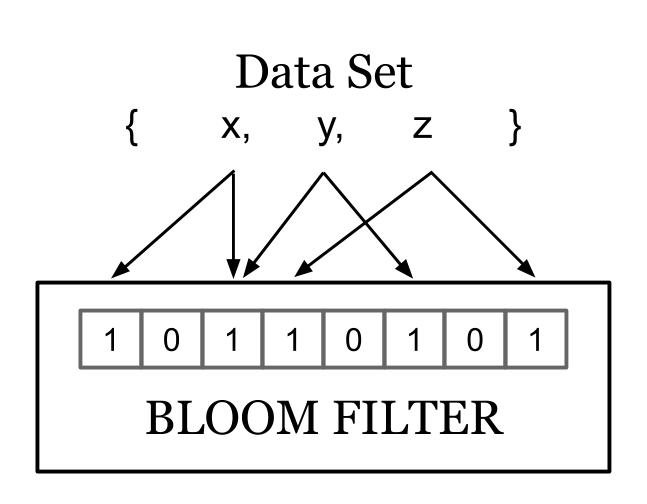
\includegraphics[width=0.5\linewidth]{Images/Diagrams/bloom_filters.png}
    \caption{Bloom filters use multiple hash functions (here just 2) to set the bits in an array. Items can be checked by hashing them and reading the contents of the array at the corresponding indices.}
    \label{fig:segwit}
\end{figure}

Bloom filters may seem very useful but, for them to be applicable to this project, I will have to include some form of identifier on each transaction. In the case of Bitcoin, the Bloom filter can simply use the addresses of the outputs to transactions. However, if I want the platform to retain more anonymity, then I will have to store something else.
This led to the development of what I call the chat identifier or \textbf{ChatID}. The ChatID is optionally\footnote{ChatID should be optional to ensure that those who want to maintain further anonymity with their messages can do so. It should be noted that the two parties should agree on this at the inception of the chat, otherwise they may miss messages that lack a ChatID.} attached, in plain text, to messages that run between users of a chat. This ChatID is decided when the two parties first make contact and maintained for the duration of the chat or until all parties unanimously agree to change it. Group chats have a single ChatID and behave identically to any other chat. Bloom filters can be included with each block when it is made and validation-checked by clients when received.

With this development, clients can now more quickly and efficiently search the blockchain for messages that are intended for them.

However, to make the idea of a ChatID more effective, it would be useful to be able to calculate the ChatID for a chat. This means it would be useful to use the keys of the sender and receiver to generate the ChatID. For now, I am using the following formula to calculate a ChatID:

\textit{TODO: The ChatID will have to be spread across the users of a group chat maybe as a kind of password??}

\paragraph{Proof of Work}
Proof-of-work is at the heart of most cryptocurrency and blockchain projects. It is an indirect way of ensuring the security of a blockchain. Normally it takes the form of a 'nonce'. A nonce is usually a number stored in the block headers. Blocks are only deemed valid if their nonce results in a Merkle hash that satisfies a certain difficulty.

Traditionally, proof-of-work is calculated by hashing the entire block using Merkle root hashes and then comparing the resulting hash to a ``difficulty'' number. If the resulting hash is lower than the difficulty value, then the block is valid. This means that the difficulty can be changed to predictably change the block-time. 



Proof-of-Work is not just applicable to blocks however, it is also used by Bitmessage on individual messages in order to discourage \textit{denial-of-service}\cite{bitmessage_pow} attacks where a user might try to rapidly send a large quantity of messages in an attempt to slow down or even halt the platform. This is a feature that I want to implement as DoS attacks could become a major problem.

The Bitmessage proof-of-work target value for individual messages is calculated as follows:

\begin{center}
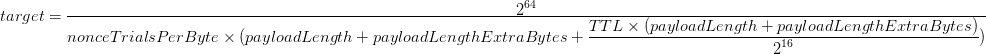
\includegraphics[width=\linewidth]{Images/Diagrams/bitmessage_pow.png}
\end{center}

This is obviously quite a large formula and relies on several variables not discussed up to this point. It uses some variables which are less relevant to the design of \textit{my} platform.

To begin with, I stripped the formula of unwanted variables such as TTL (Time-To-Live for the given message). This resulted in the following:
\begin{center}
\[\textit{target} = \dfrac{2^{64}}{\textit{payloadLength} + \dfrac{\textit{payloadLength}}{2^{16}}}\]
\end{center}

As the \textit{payloadLength}\footnote{The \textit{payloadLength} refers to the number of bytes that make up the transaction.} increases, the \textit{target} will decrease. However, with this system, the target will be too easy for small messages. This is why Bitmessage utilises message padding in the form of \textit{payloadExtraBytes}. \textit{payloadExtraBytes} is set to 1000\footnote{It should be noted that the value of \textit{payloadExtraBytes} can be tuned to change the difficulty of sending a message. }. With \textit{payloadExtraBytes} reintroduced, the formula reads:
\begin{center}
\[\textit{target} = \dfrac{2^{64}}{\textit{payloadLength} + \textit{payloadExtraBytes}  + \dfrac{\textit{payloadLength} + \textit{payloadExtraBytes}}{2^{16}}}\]
\end{center}

Unlike PoW for blocks, the target value for message transactions is not dynamically changed in Bitmessage. This means that, unless the entire protocol is updated, the difficulty value is effectively static for any given messages of the same length. I don't think that this will be realistically sustainable because if the platform were to gain real popularity in the future, then the growth in processor speed might render the DoS protection futile.

I would like the difficulty of creating a transaction to be dynamically changed to reflect the growth in computational power. To do this I need a variable that will change over time. For example, I could use the block-difficulty constant as that would grow over time with the growth of popularity and computational power. However, this example would introduce a new problem; the transaction creator would have to know in which block their transaction is to be contained ahead of time which is simply impossible. I am not sure if there is an effective solution for this but for now I am going to stick with the above formula. We can simplify\footnote{The reason why it is ok to remove the second part of the denominator is because that was just a way of scaling Bitmessage's PoW difficulty with TTL (Time-To-Live). Since there is no such thing as TTL for a transaction on my platform, this can be ignored.} this further to the following:
\begin{center}
\[\textit{target} = \dfrac{2^{64}}{\textit{payloadLength} + \textit{payloadExtraBytes}}\]
\end{center}

In the future, I hope to modify this formula to be more dynamic as discussed.

To actually calculate a PoW, a client should use the following formula (approximately same as Bitmessage):


\paragraph{Message Encryption}
To actually protect the content of messages and their respective senders and receivers, some form of encryption is necessary. The easiest method for protecting message content is to use encryption on only the message content and not on the addresses of the sender and receiver. This has the advantage of avoiding the need for a ChatID system as mentioned in paragraph \href{para:bf}{Bloom Filters} but this would obviously go against my aims for true anonymity. Using this method would result in so-called 'psuedonymity', where the users' true identities cannot be linked to their address easily except for when a malicious user analyses and cross-references their messages. As discussed in the research phase of this project, I do not believe that 'psuedonymity' is sufficient to protect users' privacy and thus I can and will not use this method.

The advent of the ChatID idea allows for a more elegant approach in which the whole transaction is encrypted (except for some metadata and the ChatID of course). This means that only the sender and receiver can see the addresses of their counterparts and not just anyone. This solution seems to me to be very effective at achieving the goals of this project and is 'tried and tested' by Bitmessage as they use a similar method with some modifications. I like the idea of this system because it makes every transaction completely unintelligible for an anyone who isn't part of the chat. Another key decision here is how to make this system work for group chats. I have already come to the conclusion that the `one-to-one' method is the way forward and therefore it makes sense for there to be only one ChatID for a group chat.

However, it is clear that some of a transaction's data must remain unencrypted. I have decided that the `version' field must remain unencrypted since the version of the platform may determine how the encrypted data is to be decrypted. It is also important because it allows clients to disclude messages with older versions from their block generation (older versions may contain insecure encryption techniques). This means that in the future, the algorithm for encryption and decryption of transactions could be changed.

Now I must decide which fields should be encrypted and which shouldn't be. Obviously the message data must be encrypted. So too must the addresses of the sender and receiver in order to preserve anonymity as discussed above. I have also concluded that some fields should not be encrypted such as the version field.

The following table shows the fields of a transaction which I believe ought to be encrypted.
\begin{table}[H]
\centering
\begin{tabular}{|p{2.5cm}|p{8.5cm}|}
\hline
\rowcolor{tblgrey}
Description & Comments              \\ \hline
msg\_id     & msg\_id of message. (Used for acknowledgements and reactions)\\ \hline
tx\_from    & Address of sender (0x0 for anonymous).                       \\ \hline
tx\_to      & Address of recipient.                                        \\ \hline
tx\_sig     & Cryptographic signature of transaction.                      \\ \hline
msg\_type   & Type of message. (text, acknowledgment, sticker...)          \\ \hline
msg         & Message object. (has different subfields depending on msg\_type) \\ \hline
\end{tabular}
\end{table}



\subsubsection{Blocks}
Blocks are fundamental to this project in that they are what separate this from other services like Bitmessage. The concept of a blockchain is inherently based around the grouping of transactions (in the case of a cryptocurrency) into blocks. The block is what differentiates a blockchain from a database and the block's proof-of-work is the backbone of trustless interaction between users of a blockchain.

The block is a relatively simple structure. It contains a section for headers which store all the metadata and a section for transactions. The headers include information such as the version of the platform that the block was created with; the number of included transactions; the proof-of-work nonce; and more. I created the following table for all the information that the headers will need to store.
\begin{table}[h]
\centering
\begin{tabular}{|l|l|}
\hline
\rowcolor{tblgrey} 
Headers    & Description                                       \\ \hline
version    & Version of platform used by block creator.        \\ \hline
nonce      & A proof-of-work nonce used for block validation.  \\ \hline
length     & The number of included transactions               \\ \hline
cid\_bloom & The bloom filter which filters according ChatID.  \\ \hline
\end{tabular}
\end{table}

These provide enough metadata to create a standalone block but I want to create a blockchain which means that I need a way of identifying a block and linking it to a previous block. I will accomplish this with Merkle root hashes.

\paragraph{Merkle Root Hashes}
Merkle root hashes are a way of hashing a large array of data such as a list of transactions. It does this by hashing neighbouring elements together, then concatenating neighbouring hashes together and hashing those. This is repeated over and over until only one hash is left (see \autoref{fig:merklert}).
\begin{figure}[h]
    \centering
    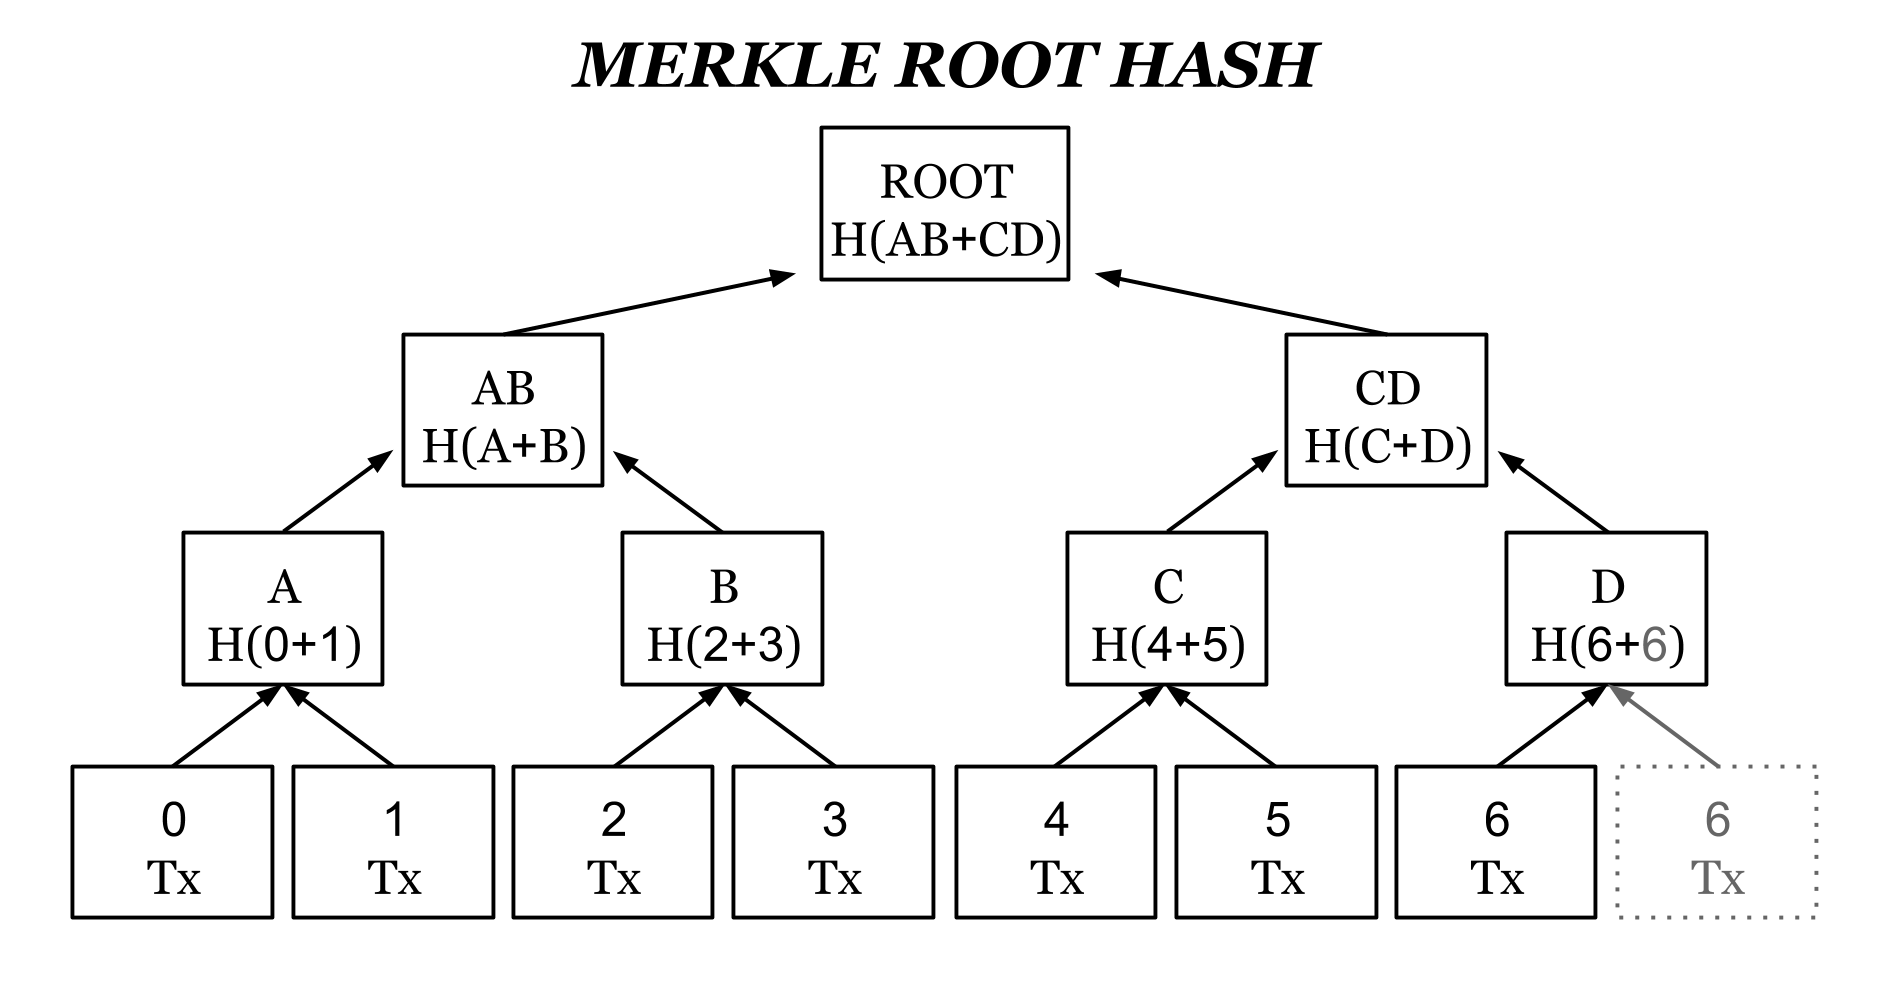
\includegraphics[width=0.95\linewidth]{Images/Diagrams/merkle_root.png}
    \caption{Merkle root hashes are calculated by recursively hashing transactions and then hashes of transactions and then hashes of hashes and so on...}
    \label{fig:merklert}
\end{figure}

Merkle hashes provide a good way of identifying blocks as they cannot be forged. It is also extremely unlikely to ever have a collision between two blocks' roots. This is ideal for identifying blocks and so I will be using this as a 'BlockID'. This can then be added to the design of a block as so:
\begin{table}[h]
\centering
\begin{tabular}{|p{2.5cm}|p{8.5cm}|}
\hline
\rowcolor{tblgrey} 
Headers    & Description                                         \\ \hline
version    & Version of platform used by block creator.          \\ \hline
merkle     & The Merkle root hash of the current block. (BlockID)\\ \hline
prev       & The hash the previous block in the blockchain.      \\ \hline
nonce      & A proof-of-work nonce used for block validation.    \\ \hline
length     & The number of included transactions.                \\ \hline
cid\_bloom & The bloom filter which filters according ChatID.    \\ \hline
\end{tabular}
\end{table}

\begin{figure}[h]
    \centering
    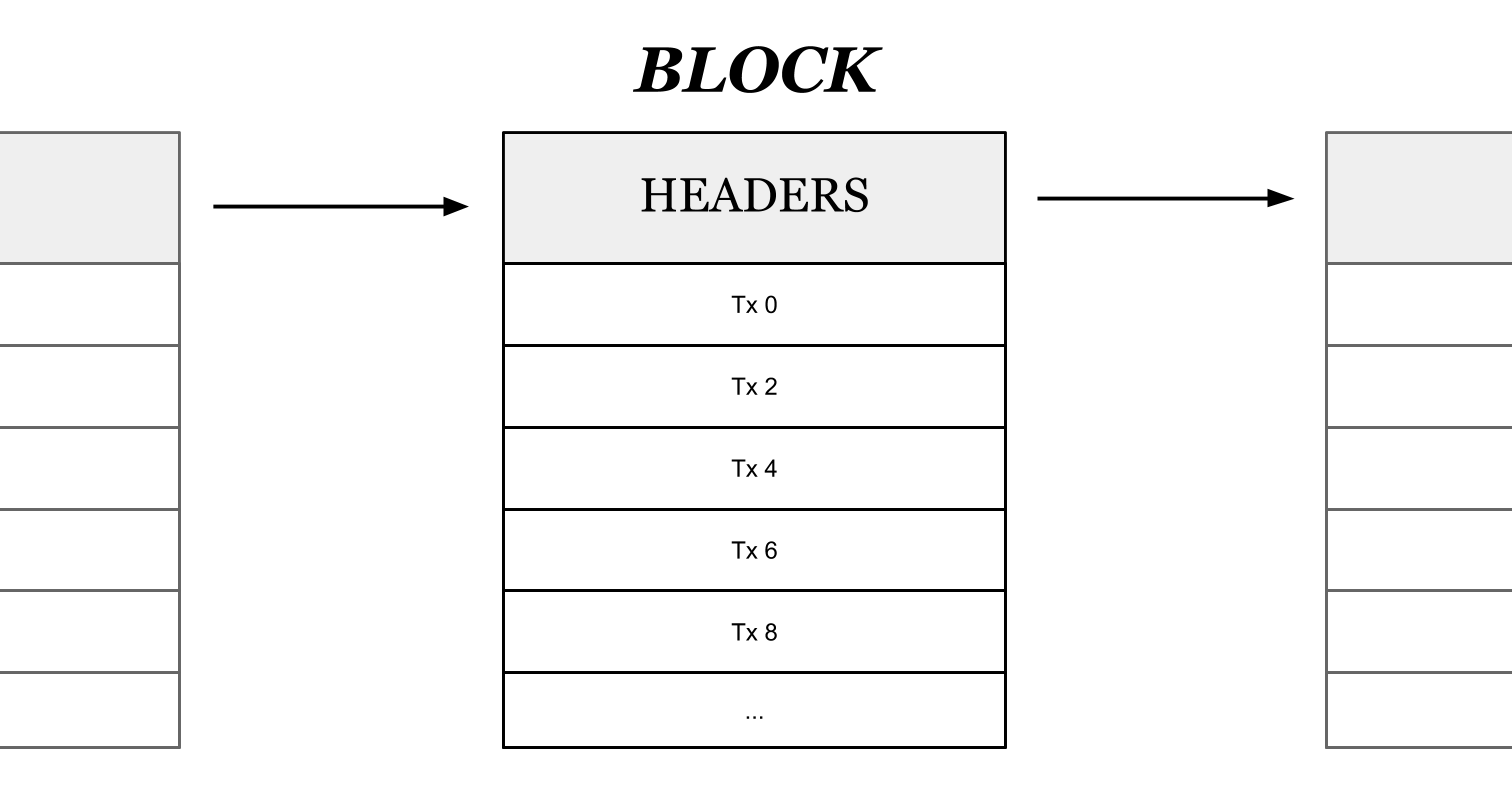
\includegraphics[width=0.95\linewidth]{Images/Diagrams/blockchain_block.png}
    \caption{A simplified diagram of the structure of a block.}
    \label{fig:block}
\end{figure}

\paragraph{Proof of Work}
I propose that the difficulty value should be computed, as in Ethereum, with the following formula where ``block\_time'' is the time between the two most recent blocks.
\[\textrm{difficulty}_{\textrm{new}} = \textrm{difficulty}_{\textrm{old}}
\ + \ \left\lfloor\dfrac{\textrm{difficulty}_{\textrm{old}}}{2048}\right\rfloor \times \max\left(1- \left\lfloor \frac{\textrm{block\_time}}{10} \right\rfloor,\ -99\right)\]

The target hash value can then be calculated as follows.
\[\textrm{target}_{\textrm{new}} = \frac{\textrm{target}_{\textrm{old}}} {\textrm{difficulty}_{\textrm{new}}}\]

\newpage
\subsection{Network Protocol V1}
This section documents the design process for the proposed network protocol. The network protocol is the 'set of rules' to be followed by all devices on the peer-to-peer network and is how different devices know how to interact with each other. This needs to be standardised for a network for obvious reasons.

\subsubsection{Underlying Protocol Layers}
The network protocol that this project builds itself relies upon many lower-level layers of protocols. This abstraction will make network design simpler and reduce the complexity of the design.

The industry standard for network communication is TCP (Transmission Control Protocol) which itself lies on top of the IP protocol. TCP is used for the majority of web communications and is the backbone of HTTP. It is well documented and supported by all major programming languages making it ideal for a network such as this. It handles many of the more difficult problems with network interaction such as packet loss and flow control. However it can be slower than other protocols due to it having these features. An alternative to TCP would be UDP (User Datagram Protocol) which is known for being better at low-latency connections than TCP but only if the sender and recipient are more tolerant of packet loss.

\newpage

\textbf{TCP}
\textit{ - Advantages}
\begin{itemize}
    \item Widely used with excellent implementation documentation. This makes for simple design and implementation and a better developer experience overall.
    \item Handles packet loss well. This is useful for this blockchain service because it means that all communications are guaranteed\footnote{In the case where a network client (sender or receiver) is disconnected from the network entirely during communications, the connection stream must be dropped and the packets will never make it to their destination.}.
\end{itemize}

\textit{ - Disadvantages}
\begin{itemize}
    \item Designed for relatively small packets and may not handle large data-sets well. When a client sends a block to another client, the network may slow down.
    \item Designed with ordering and ease-of-use in mind over speed. This could limit the rate of communications and slow down the network.
\end{itemize}


\textbf{UDP}
\textit{ - Advantages}
\begin{itemize}
    \item All-around faster protocol. Perfect for transfer of fairly large data such as a block of transactions.
    \item Fewer features means less overhead.
\end{itemize}

\textit{ - Disadvantages}
\begin{itemize}
    \item Harder to implement since doesn't automatically handle features like packet ordering and packet re-sending if any are dropped.
    \item Less well-used by the developer community and therefore often has worse support.
\end{itemize}

The obvious option here is TCP and from this point onward, that is the option that I will run with. It is worth noting that, in the future, some UDP communications could be implemented into network interactions to speed up specific requests on the network. For example, large transfers of data such as blocks could be modified to make use of UDP or something similar. Also, since it is probable that most implementations of this platform will be open source, it would be fairly easy for a developer to fork a project and create their own version which makes use of UDP or other future protocol.

\subsubsection{Network Serialisation}
Serialisation is the way objects get stored on disk and in the network. This decides the order of the fields in a network request and the number of bits assigned to each. This section will inherently overlap somewhat with disk serialisation (ie. the way blocks are stored on disk) however disk serialisation will be specific to each client implementation. If the network serialisation for the proposed network were to prioritise the wrong fields or be overly `bloated', then the network could become slow and expensive for users, taking up more network bandwidth than necessary. Likewise if the designated field sizes were to be too \textit{small}, then users may have to send more requests than necessary to the network in order to fully communicate.

To contain the data, a set of primitive data types must be defined. Here is a set of a few primitives that I know I will need.
\begin{table}[h]
\centering
\begin{tabular}{|l|p{8.5cm}|}
\hline
\rowcolor{tblgrey} 
Data Type  & Description            \\ \hline
uint\_8     & 8 bit integer.         \\ \hline
uint\_32    & 32 bit integer.        \\ \hline
uint\_64    & 64 bit integer.        \\ \hline
var\_uint   & Variable size integer. \\ \hline
uint\_xx[ ] & Array of xx-bit integers.\\ \hline
\end{tabular}
\end{table}

To store integers that are of large sizes, the variably sized integer (var\_int) consists of a byte indicating the length in bytes of the following number. This will allow for client software to decode very large numbers with no confusion over field sizes that store numbers of variable length. Likewise if the number is small, then no bytes are wasted. Since none of the data that will be used is negative, all of these integers are \textbf{unsigned}.


\textit{TODO: v2 add data types for strings. change var\_int to be like Bitmessage not counting bytes.}

\paragraph{Requests}
The structure of a request is standard for all requests. This is the lowest level defined by my specification. Bitcoin and Bitmessage have similar network request structures, essentially consisting of the following.
\begin{table}[h]
\centering
\begin{tabular}{|l|p{8.5cm}|}
\hline
\rowcolor{tblgrey} 
Field       & Description                                      \\ \hline
magic       & Magic value indicating origin network.           \\ \hline
command     & Identifies packet content (ie. encodes the purpose of the message). \\ \hline
checksum    & Checksum hash of request payload.                \\ \hline
payload     & Actual request payload (ie. content of request). \\ \hline
\end{tabular}
\end{table}

The \textbf{magic} value is a specific number that refers to the network of the request. Bitcoin has a test network that allow for developers to test their software with no real stakes. If the magic value is anything other than 1 of 2 arbitrary values\footnote{In the case of Bitcoin, the Magic values are 0xF9BEB4D9 and 0xFABFB5DA for the main and test networks respectively. They were chosen because they are unlikely to occur randomly in data.}, then the network will reject the request. This is a precaution to avoid cross-protocol confusion.

The \textbf{checksum} value is an easily-computed value that verifies that the payload is intact. This helps to reduce the possibility of erroneous or potentially incorrect data reaching a client.

The \textbf{command} value is, for Bitcoin and Bitmessage, the type of the request being made. For example Bitmessage has several different commands including `version' to indicate a client's protocol version to another device and `inv' to communicate the extent of a client's message inventory.

\paragraph{Transactions}
To serialise transactions, I will need to decide the data type for each field. For example, I will need a field for the version of the platform on which the transaction was sent. This can be stored as a uint\_8 since the platform is unlikely to receive massively frequent updates. 

\textit{TODO: v2 change version to uint\_32 or string.}

\textit{TODO: convert transaction to network object.}


\paragraph{Blocks}
Blocks are simple to serialise as they have only a few fields. In order to decide the bit-length for the `merkle' (ChatID) field and thus also the `prev' field, I calculated the number of blocks that can be used for each type of integer without overflowing. For uint\_32, the largest possible number of blocks with differing Merkle-hashes is $2^{32}$; for uint\_64, it is $2^{64}$. At a block time of \textasciicircum15 seconds, this means that the maximum possible (though unlikely) lifetime of the blockchain would be:

\[\textrm{lifetime}_\textrm{max} = \textrm{number of blocks} \times \textrm{average block time}\]

For uint\_32:
\begin{align*}
    \textrm{lifetime}_\textrm{max} &= 2^{32} \textrm{ blocks} \times 15 \textrm{ seconds} \\
    &= 64424509440 \textrm{ seconds} \\
    &= 745654 \textrm{ days} \\
    &= 2042 \textrm{ years}
\end{align*}

For uint\_64:
\begin{align*}
    \textrm{lifetime}_\textrm{max} &= 2^{64} \textrm{ blocks} \times 15 \textrm{ seconds} \\
    &\approx 2.767e20 \textrm{ seconds} \\
    &= 3.203{\times}10^{15} \textrm{ days} \\
    &= 8.774{\times}10^{12} \textrm{ years}
\end{align*}

Since the scale of both is huge, I have decided to use uint\_32 here at least for V1.

\textit{TODO: v2 change merkle to char[32]}
\textit{TODO: v2 bloom filter service can respond with headers array instead of bloom filter directly (maybe but kinda flawed actually).}


\begin{table}[h]
\centering
\begin{tabular}{|l|l|}
\hline
\rowcolor{tblgrey} 
Field           & Data Type \\ \hline
version         & uint\_8   \\ \hline
merkle          & uint\_32  \\ \hline
prev            & uint\_64  \\ \hline
nonce           & uint\_32  \\ \hline
length          & uint\_32  \\ \hline
cid\_bloom      & uint\_64  \\ \hline
\end{tabular}
\end{table}

\clearpage
\printbibliography
\end{document}
